\hypertarget{criterion-8-continual-quality-improvement}{%
\chapter{Criterion 8: Continuous Quality Improvement (CQI)}\label{criterion-8-continual-quality-improvement}}

\hypertarget{sec:9.1general-nust-quality-enhancement-cell}{%
\section{General -- NUST Quality Enhancement Cell}\label{general-nust-quality-enhancement-cell}}

Lately, the realization of the need for quality assurance in higher education has become a global phenomenon. NUST also felt the need to assess and improve the quality of higher education in the country, with the objective of achieving international competitiveness and compatibility of its academic programs and research quality. Considering this NUST Quality Assurance Directorate takes care of quality assurance policies in all institutions of NUST. Organizational structure of NUST Quality Assurance (QA) Directorate is illustrated in Figure~\ref{fig:sample}.
\begin{figure}[h]
    \centering
    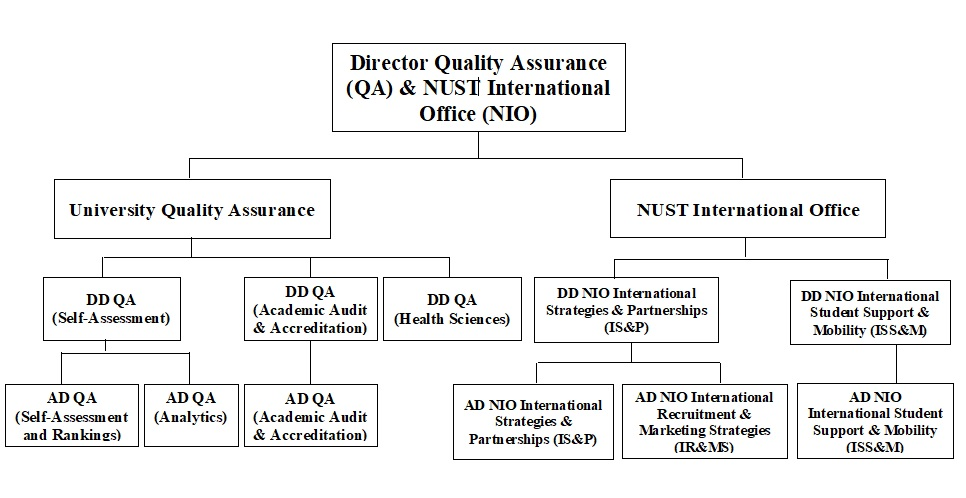
\includegraphics[width=0.8\textwidth]{images/criterion_8/media/nustqa.jpg}
    \caption{Organizational structure of NUST Quality Assurance Directorate}
    \label{fig:sample}
\end{figure}


One of the tasks of NUST QA is the academic quality audit of all the programs at NUST that carried out annually or periodically as deemed necessary, to ensure quality of program and identify any flaw and drawbacks in the program. The NUST Quality Assurance Directorate is committed to ensuring excellence in education and research by implementing a comprehensive quality assurance framework aligned with national and international standards. Its vision is to deliver high-quality education that is globally competitive, while its mission focuses on developing and implementing quality assurance policies, building faculty and staff capacity, conducting systematic assessments and audits, enhancing academic quality, and promoting internationalization. The Directorate's objectives include implementing the Higher Education Commission's quality assurance framework, conducting self-assessment and internal quality audits, ensuring compliance with accreditation requirements, improving teaching, research, and support services, strengthening institutional capacity, supporting university rankings through data management, fostering national and international collaborations, and contributing to quality enhancement in higher education. Established in 2005 as one of the first Quality Enhancement Cells under the HEC initiative, the QA directorate adopts a holistic, continuous quality improvement approach centered on self-assessment, evidence-based evaluation, and institutional excellence.


\hypertarget{local-quality-enhancement-cell-lqec}{%
\section{Local Quality Enhancement Cell (LQEC)}\label{local-quality-enhancement-cell-lqec}}

To ensure the effective implementation of Continuous Quality Improvement (CQI), the Department has designated the Director Local Quality Enhancement Cell (DLQEC) as the focal person for coordinating quality assurance and continuous improvement activities. The CQI Committee, headed by the Head of Department (HoD), provides oversight of the CQI process by reviewing assessment and feedback data, evaluating the corrective actions proposed by the DLQEC, recommending additional improvement measures where required, and monitoring the implementation and effectiveness of the approved actions. Through this process, the committee ensures that quality enhancement initiatives are systematically implemented and continuously monitored across the program. The structure of the CQI Committee is shown in Figure~\ref{fig:sample1}.
\begin{figure}[h]
    \centering
    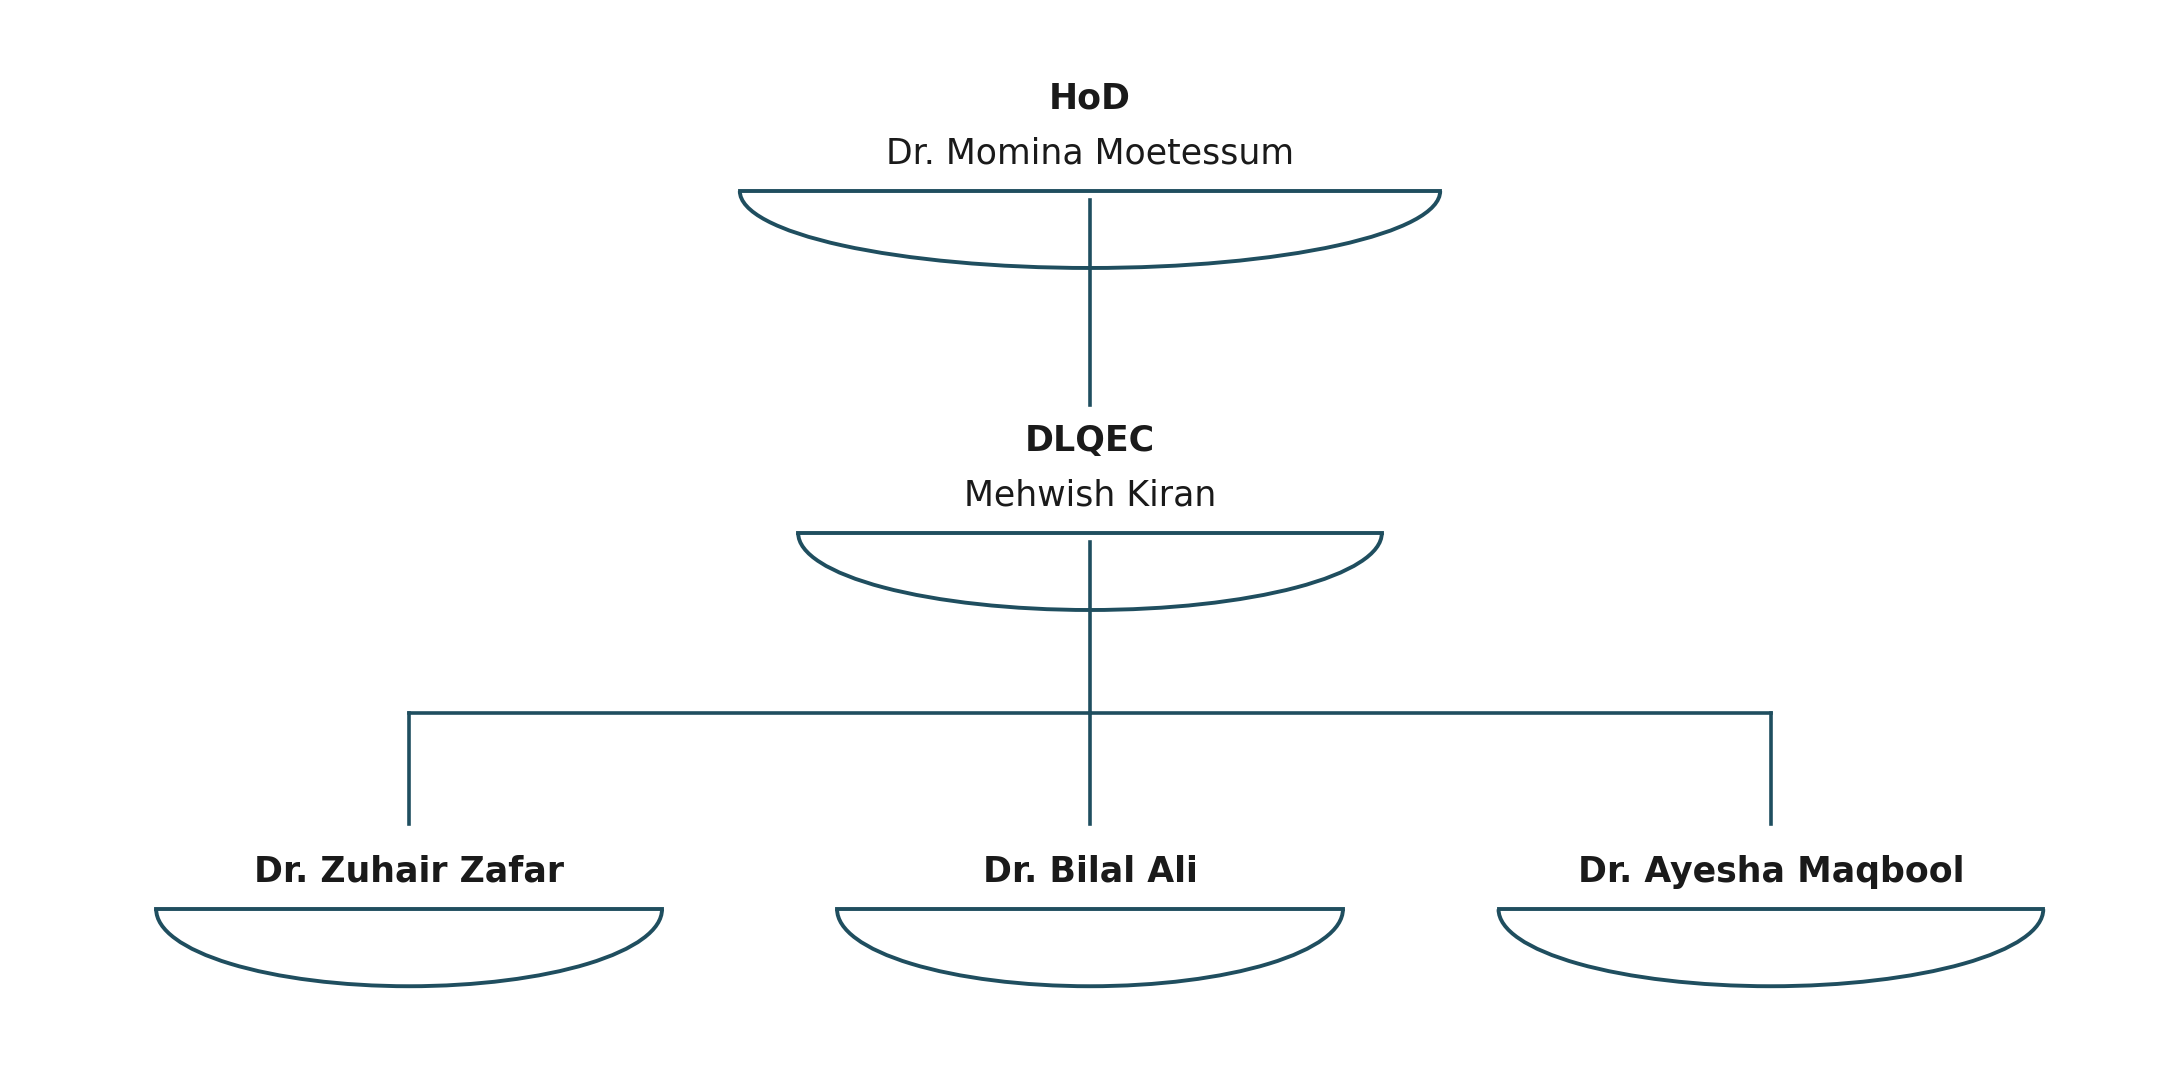
\includegraphics[width=0.8\textwidth]{images/criterion_8/media/Figure_9.2_CQI_Committee_Structure.png}
    \caption{CQI Committee Structure}
    \label{fig:sample1}
\end{figure}

For program accreditation, the DLQEC coordinates the preparation of the SAR and supports SEECS in all activities related to accreditation readiness. The DLQEC also assists in organizing the required documentation, coordinating with relevant stakeholders, and facilitating the Institute's preparations for the accreditation visit and presentations to the members of the accreditation team. The observations made during the accreditation visits are also scrutinized by CQI Committee and is responsible for implementation of any points or concerns raised during the visit. Last PEC visit was carried out in October/November 2023 and the observations with their replies are given in (Rejoinder) Annexure~\ref{annex:rejoinder}.

\hypertarget{program planning}{%
\section{Program Planning}\label{Program Planning}}
Program planning is conducted through a structured and collaborative process to ensure the effective delivery of academic, laboratory, and co-curricular activities throughout the academic year. 
At the beginning of each academic year, an annual academic plan is developed in alignment with the university's academic calendar, outlining key activities such as semester commencement, examinations, curriculum review meetings,  accreditation-related tasks, faculty development programs, industrial visits, seminars, and CQI activities. Sample for academic calendar is shown at Annexure~\ref{annex:planner}.

Prior to the commencement of each semester, detailed semester planning is carried out, including the finalization of course offerings, class schedules, examination timelines, and student advising activities. Resource planning is undertaken to ensure the availability of classrooms, laboratories, software licenses, computing facilities, and other teaching resources required for the smooth execution of academic activities by Academic Coordination Branch (ACB) and IT department.

Faculty allocation is performed based on faculty expertise, teaching workload, specialization, and previous teaching experience to ensure effective course delivery while maintaining a balanced distribution of responsibilities. Laboratory planning includes the review of laboratory manuals, preparation of equipment, software installation, procurement of consumables, scheduling of laboratory sessions, and assignment of laboratory instructors to support practical learning outcomes.

Final Year Design Project planning is initiated well before the start of the academic session through the identification of research domains, allocation of supervisors according to expertise, proposal evaluation, milestone scheduling, progress monitoring, and final project evaluations. The overall planning process is regularly reviewed through departmental meetings and feedback mechanisms, enabling timely adjustments and ensuring continuous improvement in academic quality and program effectiveness.

\hypertarget{cqi-process-in-obe-implementation}{%
\section{CQI Process in OBE Implementation}\label{cqi-process-in-obe-implementation}}

The Department of Software Engineering has established a comprehensive Continuous Quality Improvement framework to ensure the continuous enhancement of its curriculum and Outcome-Based Education implementation. The framework comprises four interconnected CQI processes covering the curriculum, CLOs, PLOs, and PEOs. The CQI model is shown in Figure~\ref{fig:sample2}. Each process follows a systematic cycle of data collection, evaluation, review, and implementation of corrective actions, ensuring that assessment results are effectively utilized to improve academic quality and maintain compliance with HEC and PEC requirements.
\begin{figure}[h]
    \centering
    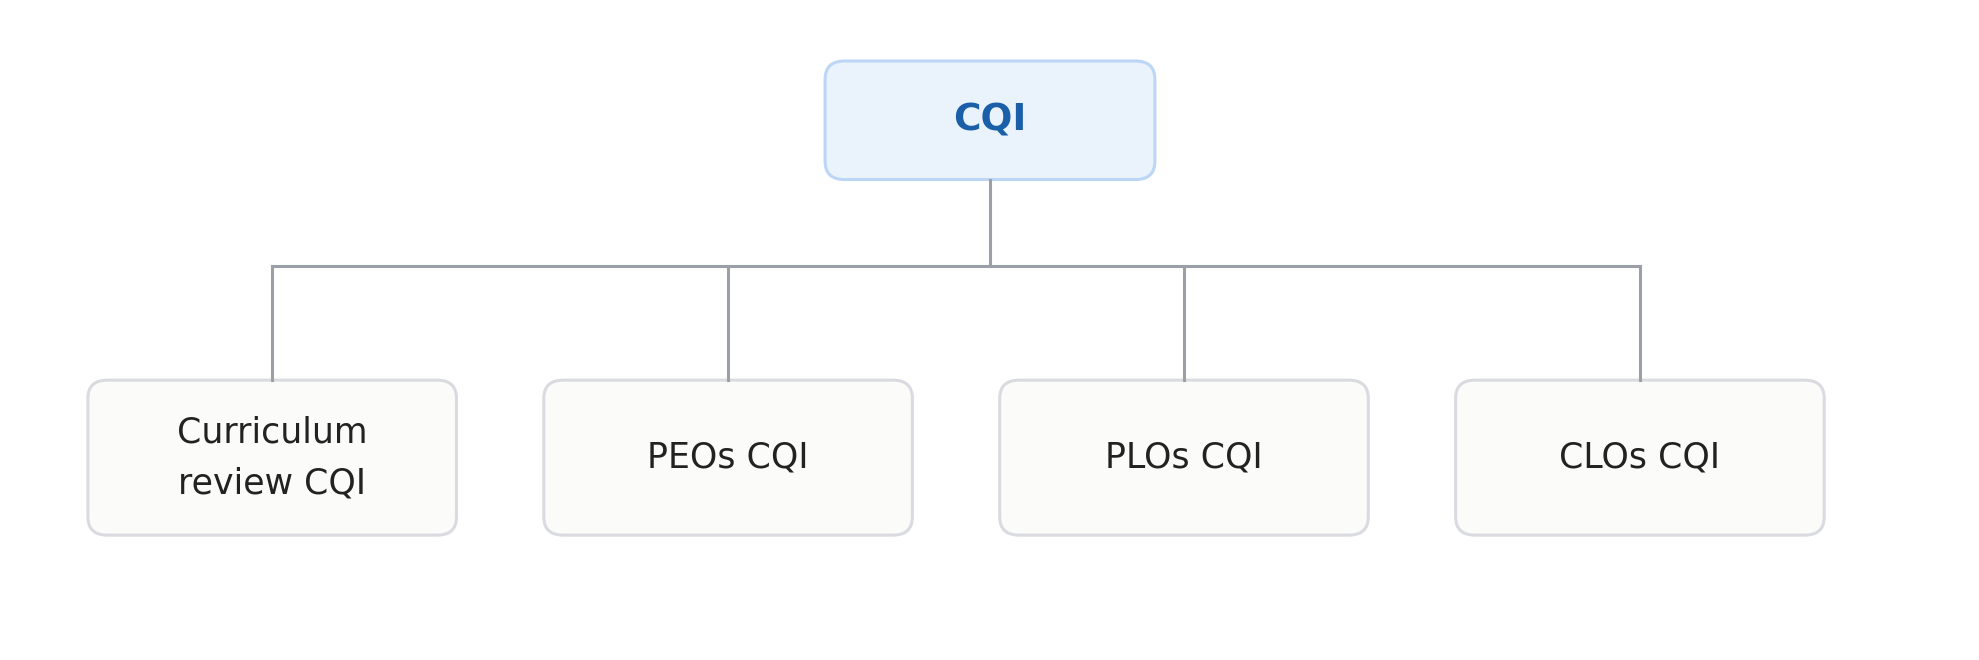
\includegraphics[width=0.8\textwidth]{images/criterion_8/media/cqi_flow.png}
    \caption{CQI Model of Software Engineering Department}
    \label{fig:sample2}
\end{figure}


To ensure that the curriculum remains relevant, effective, and aligned with evolving academic standards, technological advancements, industry requirements, and stakeholder expectations, the department follows a structured Curriculum CQI process. The process involves systematic collection and analysis of feedback from key stakeholders, review of academic performance and assessment outcomes, and consideration of regulatory and accreditation requirements. Based on this analysis, recommendations for improvement are formulated, reviewed through the appropriate academic forums, and implemented in subsequent curriculum revisions, thereby ensuring the continuous enhancement of the program.

The CQI process for CLOs, PLOs, and PEOs is illustrated in Figure~\ref{fig:sample3} through three interconnected loops. 
\begin{figure}[h]
    \centering
    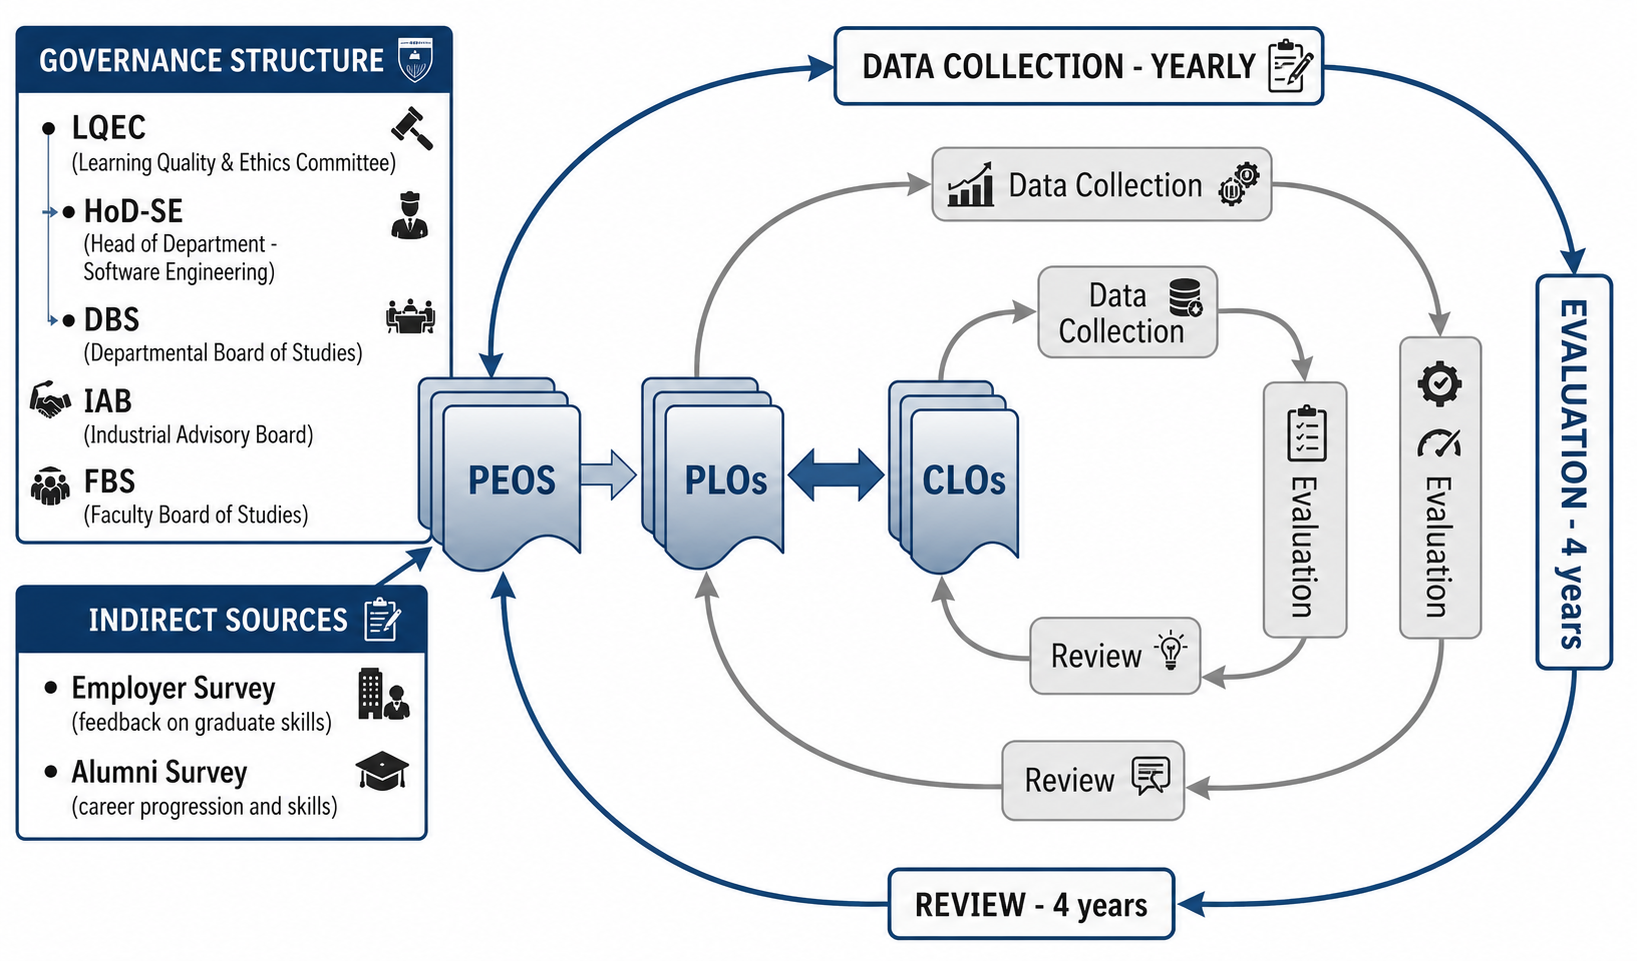
\includegraphics[width=0.8\textwidth]{images/criterion_8/media/peo-evaluation.png}
    \caption{CQI Process for CLOs, PLOs and PEOs}
    \label{fig:sample3}
\end{figure}
The innermost loop focuses on CLO attainment, which is evaluated at the end of each semester using direct assessment methods. The results are documented in Course Review Reports and corrective actions related to teaching strategies, assessment methods, or course content are implemented where required. CLO attainment forms the primary evidence for the direct assessment of PLOs, while indirect evidence is obtained through graduate exit survey and internship feedback forms. PLO attainment is reviewed after every semester to identify improvement opportunities in curriculum, teaching, and assessment practices. The outermost loop evaluates the achievement of PEOs using indirect assessment method which includes feedback from alumni and employers, typically four years after graduation. The collected data is analyzed and evaluated, and if required, corrective actions are initiated through a corrective action form as shown at Annexure~\ref{annex:corrective}. CQI for curriculum and the OBE implementation model for PEOs, PLOs and CLOs are described separately in the following paragraphs.
\hypertarget{criterion-8-Curriculum }{%
\section{Curriculum}\label{criterion-8-curriculum}}

The Department has established a systematic and evidence-based curriculum review mechanism as part of its CQI framework. The mechanism ensures that the curriculum remains current, relevant, and aligned with the requirements of the PEC, HEC, emerging technological developments, and the expectations of academia and industry. Curriculum improvements are driven through periodic evaluation of assessment data and structured stakeholder feedback, and are implemented following the University's prescribed approval process.
\hypertarget{criterion-8-CQI Process for Curriculum}{%
\subsection{CQI Process for Curriculum}\label{cqi-process-for-curriculum}}
Figure~\ref{fig:sample4} illustrates the Curriculum CQI process followed by the Department to ensure that the curriculum remains current, outcome-based, and aligned with the requirements of HEC, PEC, industry, and other stakeholders. The process begins with the collection of curriculum and course-related data from the departmental database, together with feedback from students, faculty, alumni, employers, the Industrial Advisory Board (IAB), and regulatory bodies. These inputs are reviewed by the DLQEC and subsequently evaluated by the HOD and Departmental Board of Studies (DBS), where recommendations for curriculum improvement are formulated. Proposed revisions are then processed through the university's approval hierarchy. Changes involving up to 10\% of the curriculum are approved by the Faculty Board of Studies (FBS), while revisions involving more than 10\% and up to 50\% require approval from the University Curriculum Review Committee (UCRC). Major curriculum revisions involving more than 50\% of the curriculum are submitted to the Academic Council (AC) for approval. Once the required approvals are obtained, the revised curriculum is implemented and updated in the departmental database, thereby completing the CQI cycle and ensuring the continuous improvement of the academic program.

\begin{figure}[h]
    \centering
    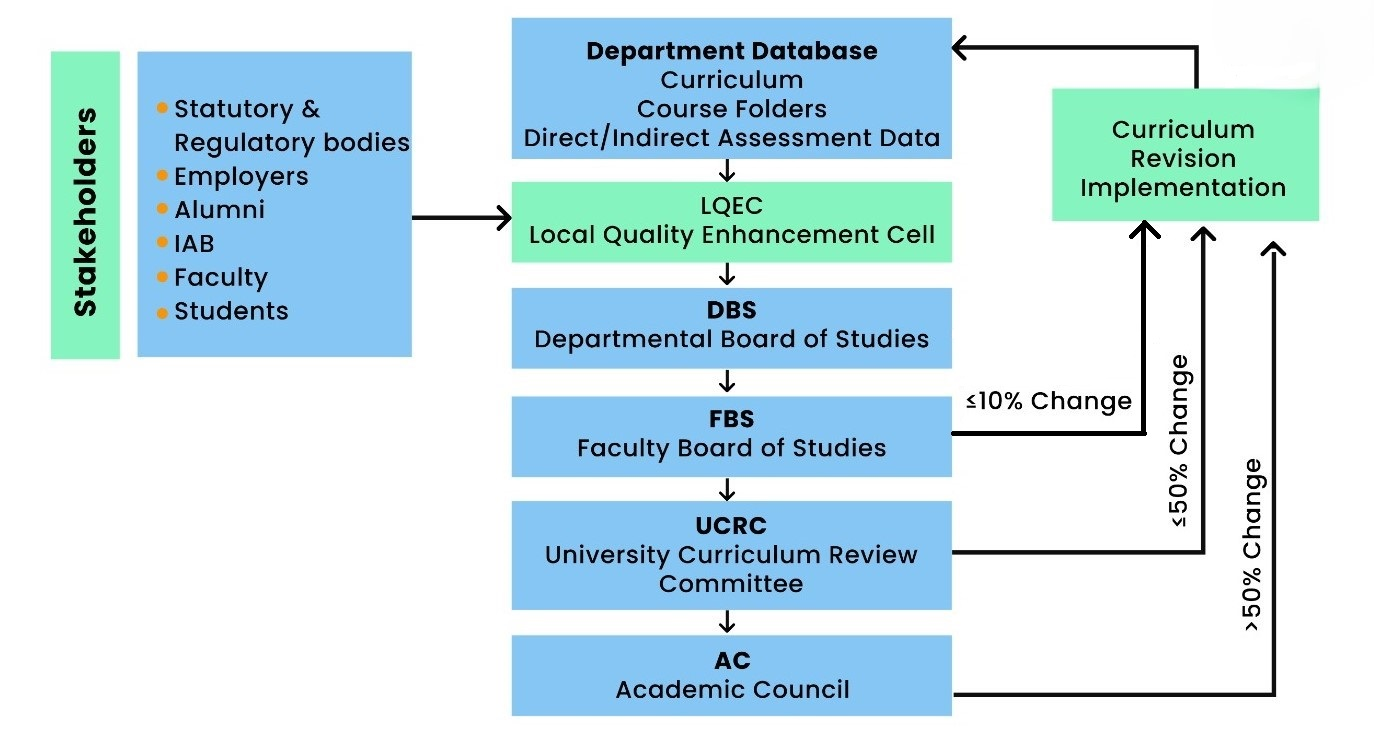
\includegraphics[width=0.8\textwidth]{images/criterion_8/media/Curr_review.jpeg}
    \caption{Curriculum Review Process}
    \label{fig:sample4}
\end{figure}

\hypertarget{criterion-8-Corrective Actions for Curriculum}{%
\subsection{Corrective Actions for Curriculum}\label{criterion-8-corrective-actions-for-curriculum}}

Table~\ref{tab:cqi_actions1} shows few corrective actions taken to improve the curriculum
\begin{table}[ht]
\centering
\footnotesize
\setlength{\tabcolsep}{4pt}

\begin{tabular}{
>{\raggedright\arraybackslash}p{4cm}
>{\raggedright\arraybackslash}p{2cm}
>{\raggedright\arraybackslash}p{3cm}
>{\raggedright\arraybackslash}p{2.8cm}
>{\raggedright\arraybackslash}p{3cm}
}
\toprule
\textbf{Observation} &
\textbf{Source} &
\textbf{Decision} &
\textbf{Action Taken} &
\textbf{Evidence} \\
\midrule
Need more software engineering electives &
IAB \& PEC  &
Added extra elective &
Updated Curriculum &
Working Paper in Annexure~\ref{annex:wp2025} \\

Inclusion of New Courses &
PEC and HEC &
Inclusion of Fehm-ul-Quran \& Pak Studies &
Updated Curriculum &
Working Paper Annexure~\ref{annex:wp2024}  \& ~\ref{annex:wp2025}  \\

Faculty Load &
HnS Faculty &
Swap Courses across semester &
Updated Scheme &
Curriculum \\

Topic Addition in Course Outline &
IAB &
Inclusion of the new topics &
Added "Rest API" in Web Engineering.  &
Course Outline \\
\bottomrule
\end{tabular}
\caption{Examples of CQI Actions}
\label{tab:cqi_actions1}
\end{table}

\hypertarget{criterion-8-peos}{%
\section{PEOs}\label{criterion-8-peos}}

\hypertarget{criterion-8-cqi-process-for-peos}{%
\subsection{CQI Process for PEOs}\label{criterion-8-cqi-process-for-peos}}

The DLQEC is responsible for the initiation of CQI for attainment, revision, and improvement of PEOs. CQI committee reviews the corrective actions to meet the desired criteria. The process of CQI for PEOs is shown in Figure~\ref{fig:sample5}. PEOs are indirectly assessed through alumni and employer surveys, where the data is collected yearly, with evaluation and review carried out four years after graduation of each batch. 

\begin{figure}[h]
    \centering
    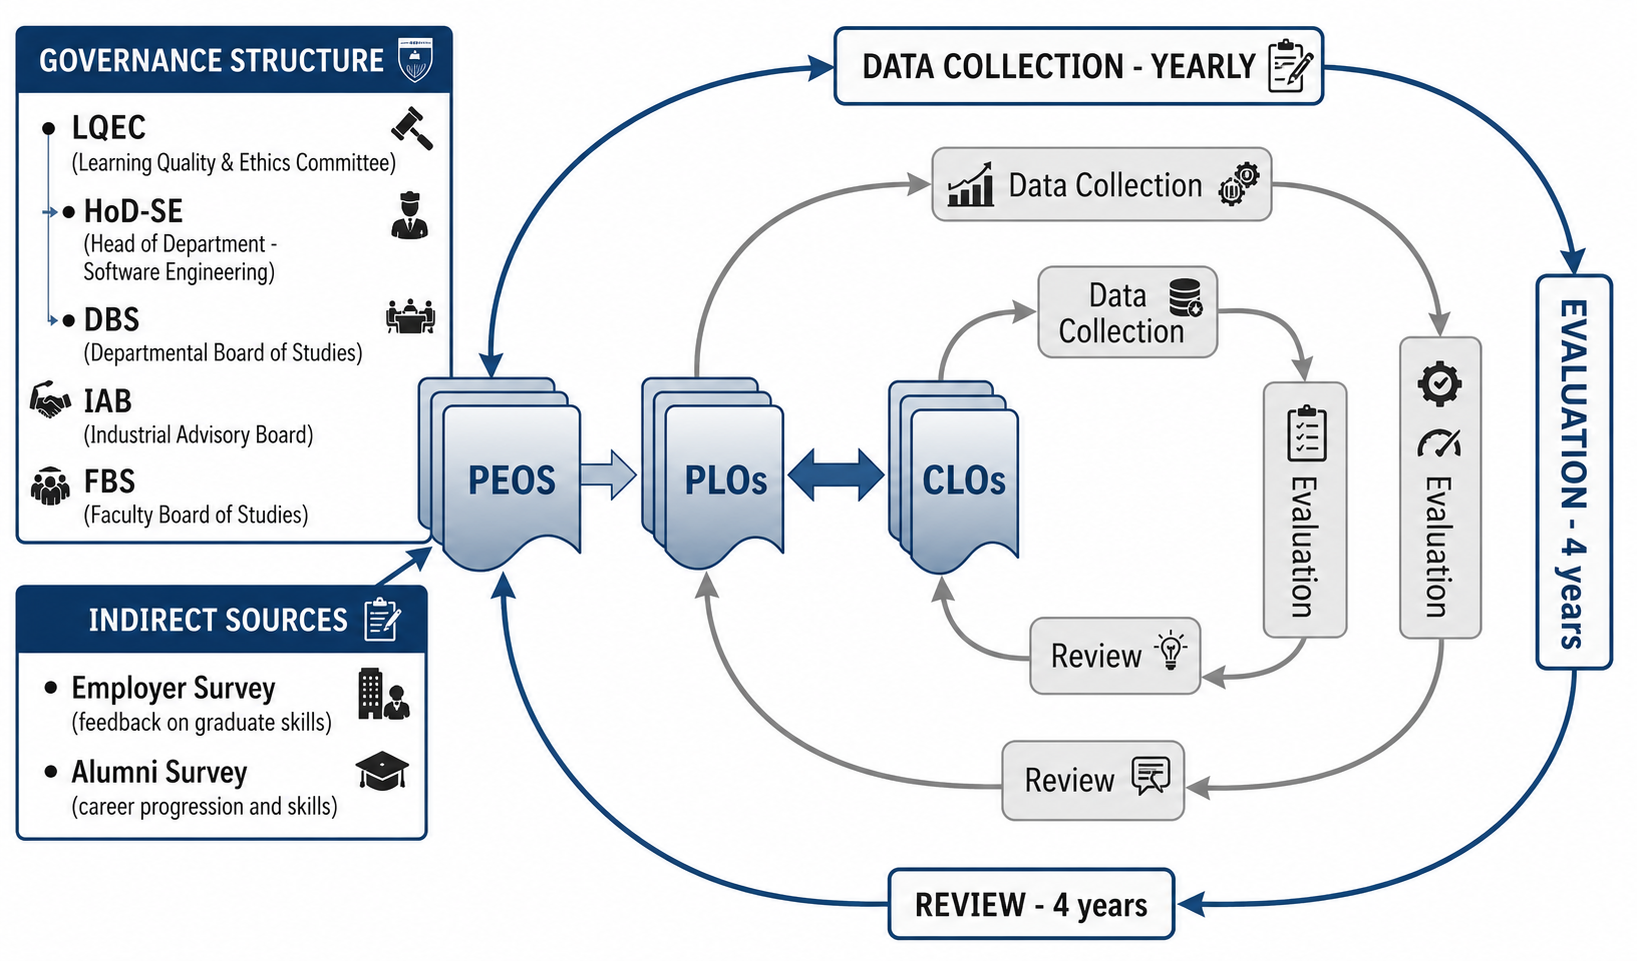
\includegraphics[width=0.8\textwidth]{images/front_matter/media/image13.png}
    \caption{CQI Process for PEOs}
    \label{fig:sample5}
\end{figure}


\hypertarget{criterion-8-review-processe-for-peos}{%
\subsection{Review Process for PEOs}\label{criterion-8-review-processe-for-peos}}

The review process starts with the measurement of PEOs and involves CQI, corrective actions, and administrative processes for the maintenance and/or improvement of PEO as shown in Figure~\ref{fig:sample6}. If the achievement of PEO is achieved, no corrective action is required; otherwise, DLQEC.invokes the CQI process. The CQI process leads to one or more corrective actions namely, revision of PEOs, revision of KPIs for PEOs, revision of assessment methods, and/or revision of curriculum/strategies. Any corrective actions if required are initiated by DLQEC and reviewed by CQI committee and may progressively be taken up to AC as mentioned previously in Criteria 1.

\begin{figure}[ht]
\centering
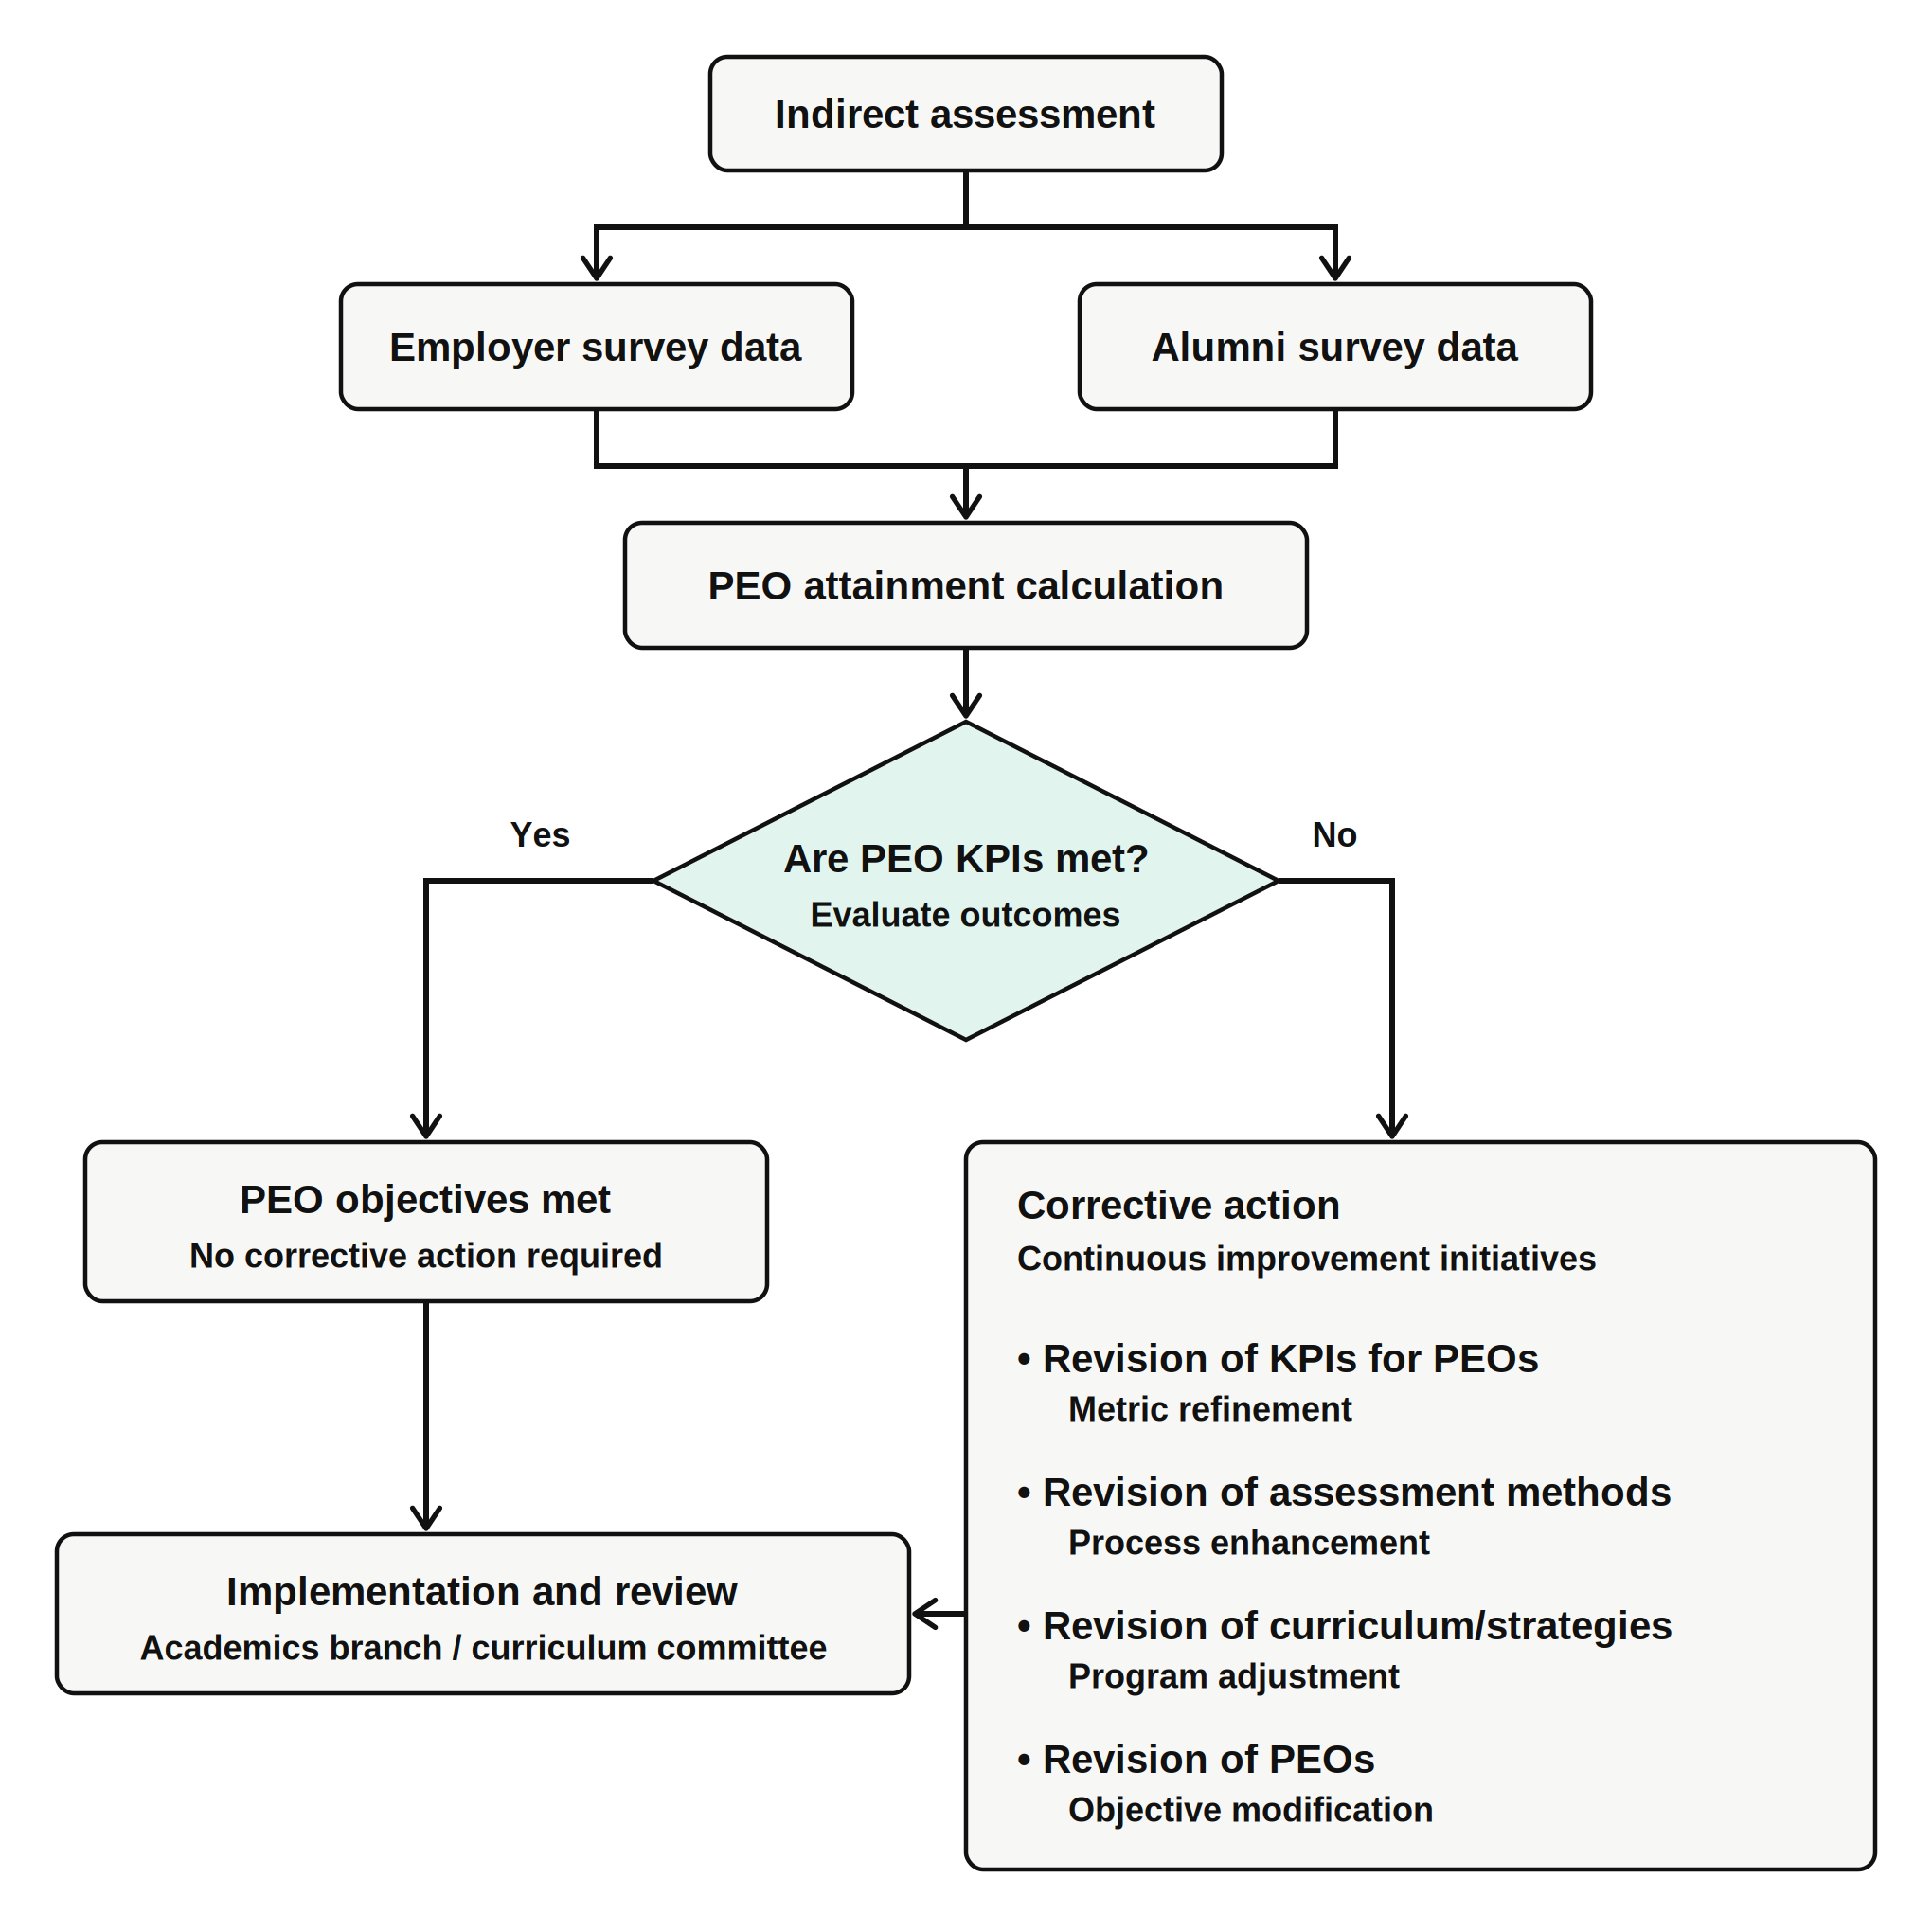
\includegraphics[width=0.89\textwidth]{images/front_matter/media/image-14.png}
\caption{Flowchart Showing Review \& Corrective Action Processes for PEOs}
\label{fig:sample6}
\end{figure}

\hypertarget{criterion-8-corrective-actions-for-peos}{%
\subsection{Corrective Actions for PEOs}\label{criterion-8-corrective-actions-for-peos}}

Figure~\ref{fig:sample7} presents the attainment of each KPI for the PEOs under the legacy evaluation system for data collected in 2025. The dashed line in each graph represents the required attainment threshold (50\% or 60\%, depending on the KPI). The result show that all KPI achieved their respective thresholds, except PEO-1, KPI-6 (pursuing higher education), which did not meet the required 50\% attainment threshold.

\begin{figure}
    \centering
    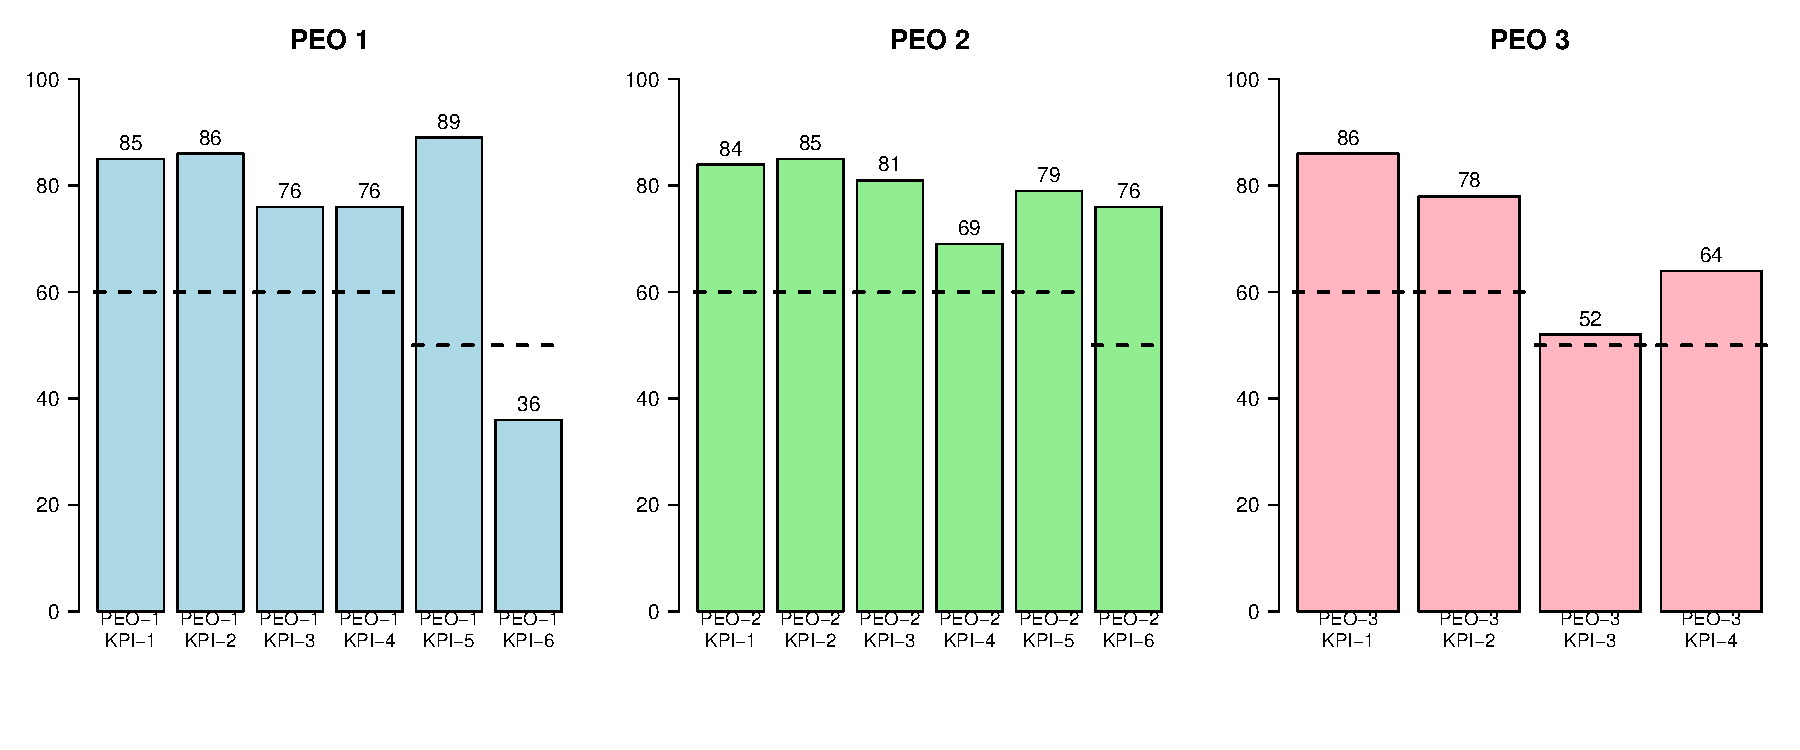
\includegraphics[width=0.8\textwidth]{images/criterion_1/media/legacy_analysis.pdf}
    \caption{Per-KPI attainment under the Legacy Evaluation System (data collected in 2025)}
    \label{fig:sample7}
\end{figure}

After analysis, the CQI committee concluded that the only KPI that did not meet the required threshold highlights a limitation of the legacy evaluation system rather than a weakness in the program. The indicator "pursuing higher education" is based on a simple yes/no outcome and does not fully reflect the achievement of the corresponding PEO. Graduates who choose to start their professional careers instead of pursuing higher studies should not be considered to have failed to achieve the goal. This limitation, along with the use of indicators that were not closely aligned with the PEOs and a rigid pass/fail evaluation approach, led to the development of the revised evaluation system described earlier.

As a result, the assessment tools to measure PEOs attainment i.e The Alumni Survey form and The Employer Survey forms were revised. Subsequently the KPIs were also revised. The revised survey forms are attached in Annexure~\ref{annex:alumni} and Annexure~\ref{annex:employer}.
\hypertarget{criterion-8-plos}{%
\section{PLOs}\label{criterion-8-plos}}

\hypertarget{criterion-8-cqi-process-for-plos}{%
\subsection{CQI Process for PLOs}\label{criterion-8-cqi-process-for-plos}}

DLQEC is responsible for CQI process for evaluation and attainment of PLOs with its designed loop shown in Figure~\ref{fig:cqi-plo} PLOs are directly assessed through CLOs and final year projects whereas indirect assessment is done through internship feedback and exit surveys. The data is collected, evaluated, and reviewed at the end of each academic semester. The entire process of review and corrective actions for the attainment of PLOs is explained in the following section.

\begin{figure}[H]
\centering
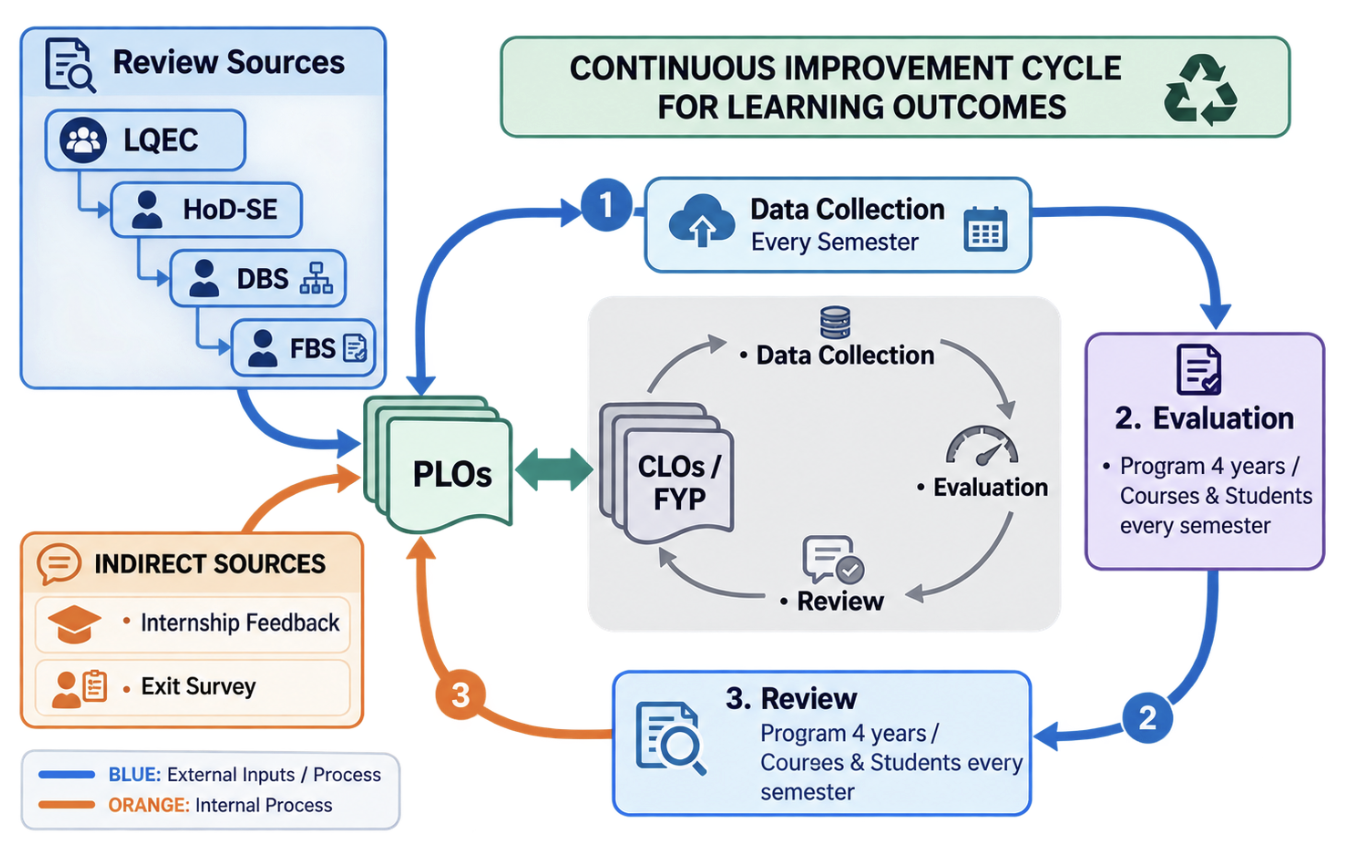
\includegraphics[width=0.88\textwidth]{images/front_matter/media/image-15.png}
\caption{CQI Process for PLOs}
\label{fig:cqi-plo}
\end{figure}

\hypertarget{criterion-8-review-process-for-plos}{%
\subsection{Review Process for PLOs}\label{criterion-8-review-process-for-plos}}


Figure~\ref{fig:individual-level} and Figure~\ref{fig:cohort-level} show the review process that starts with measurement of PLOs and involves corrective actions and administrative processes for maintenance and/or improvement of PLOs for individual as well as the cohort.  The attainment of PLOs is assessed from courses, final year design projects, internship feedback and exit surveys.  For individual students, if PLOs are attained, no corrective action is required as shown in Figure~\ref{fig:individual-level}. However, if an individual is not passing the PLOs different strategies are adopted for improvement. If an individual is not passing the PLOs in 4th – 6th semester, he/she will be counselled by the UG coordinator or student advisor, and a letter of advisory will be given to the student. If an individual does not pass PLO(s) in the 7th semester, a warning letter is issued to him. Lastly, if an individual does not pass PLO(s) in the 8th semester, a warning letter is handed to him and the department will give an extra module in the form of assignment, project study, case study, etc. to attain the deficient PLOs.


\begin{figure}[H]
\centering
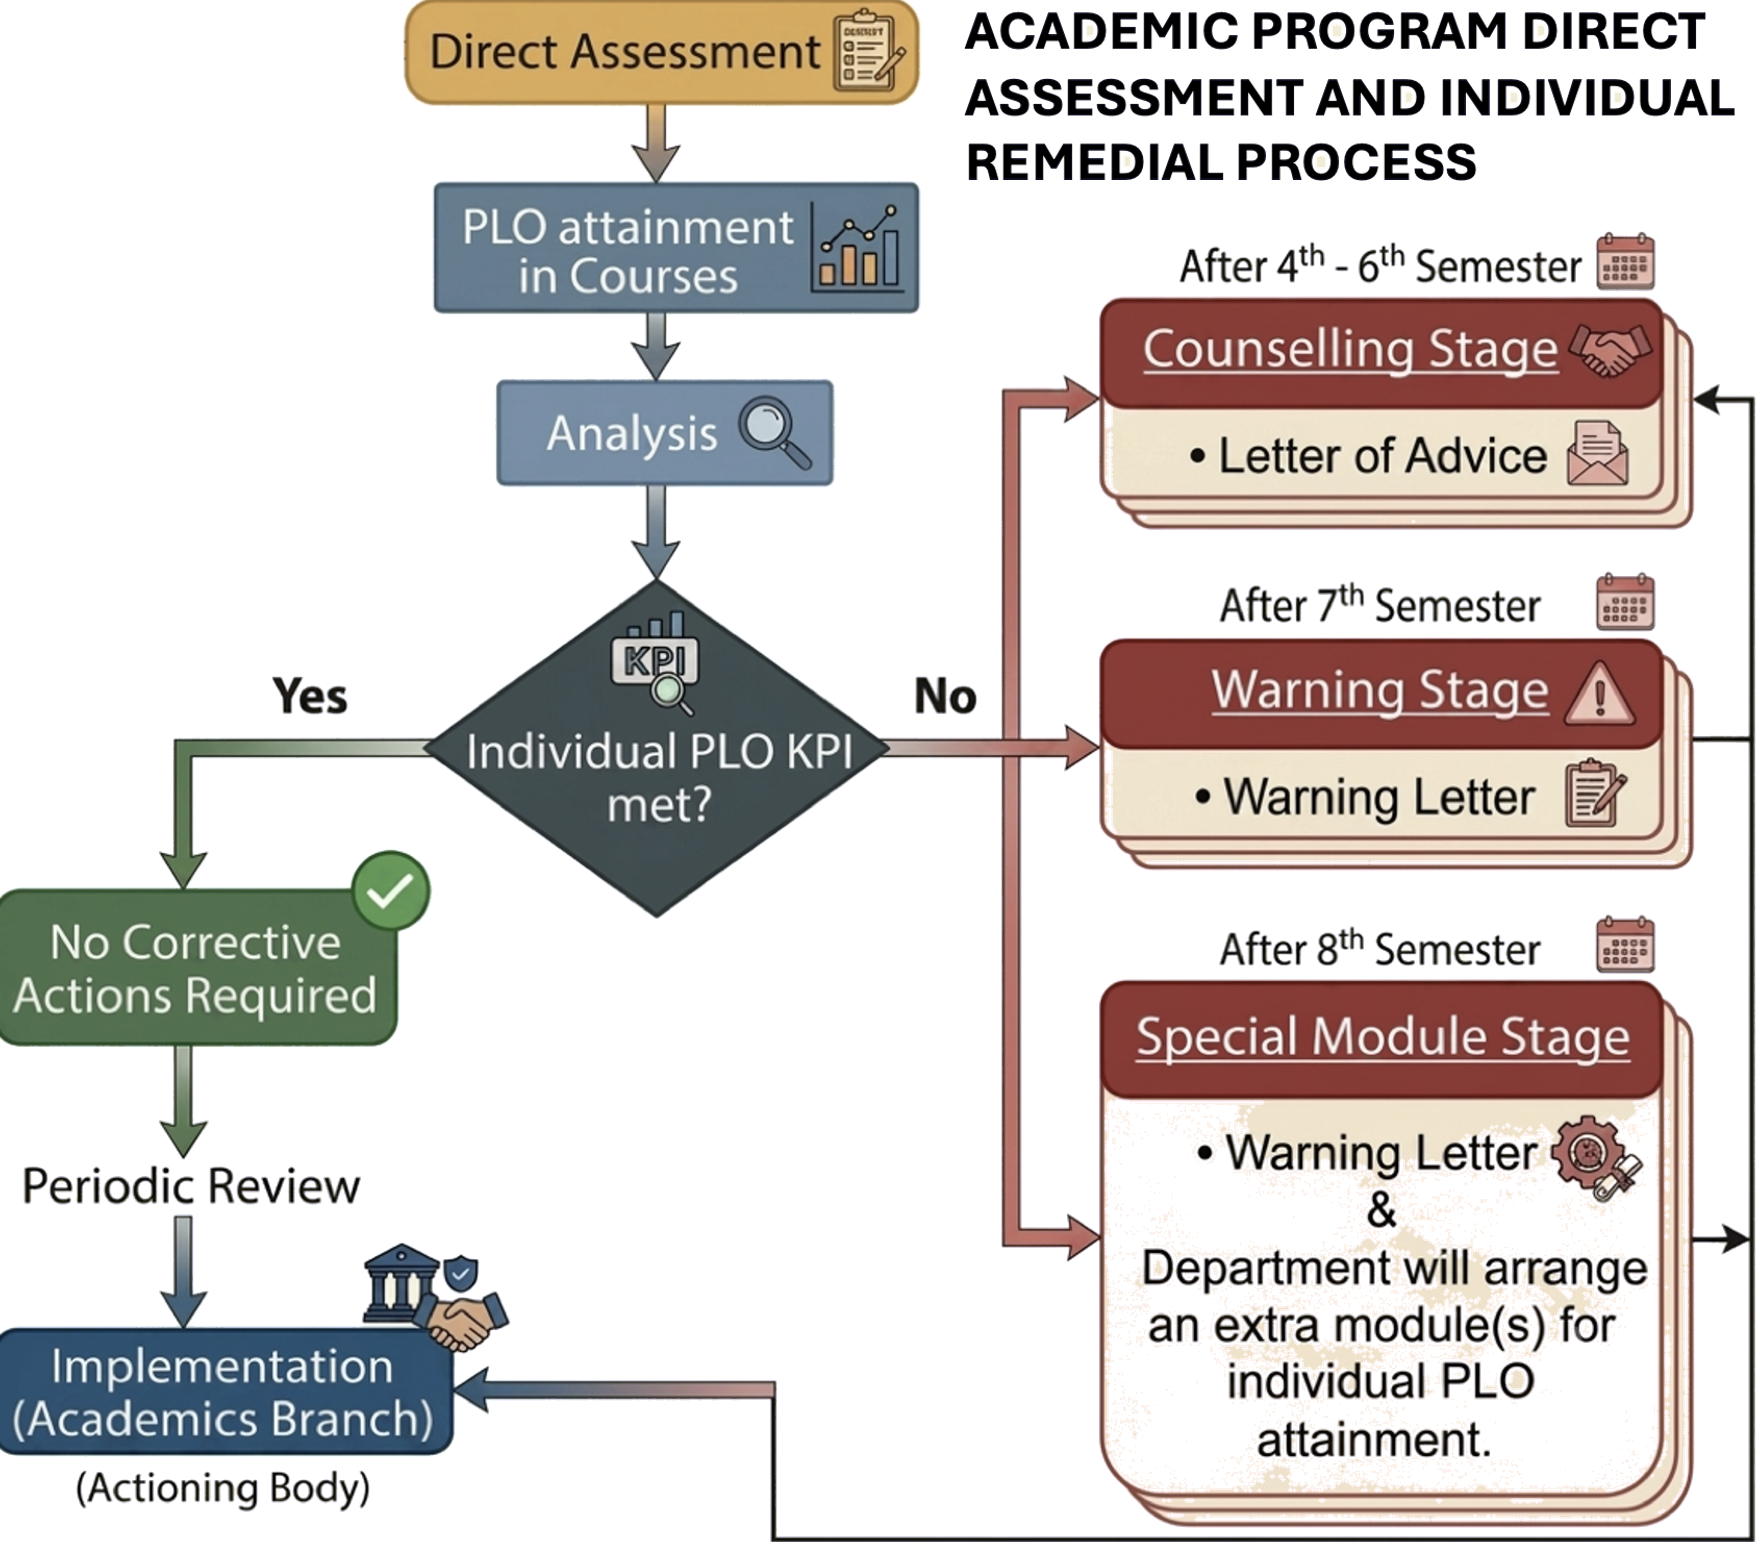
\includegraphics[width=0.7\textwidth]{images/front_matter/media/image-16.png}
\caption{Review of PLOs at Individual Level \& Corrective Actions}
\label{fig:individual-level}
\end{figure}

\begin{figure}[H]
\centering
\includegraphics[width=0.8\textwidth]{images/front_matter/media/image17.png}
\caption{Review of PLOs at Cohort Level \& Corrective Actions}
\label{fig:cohort-level}
\end{figure}

For cohort, if the PLOs attainment is more than or equal to 60 per cent as per KPI of each assessment, no corrective action is required.  However, if PLOs attainment is less than 60 per cent, the CQI process invokes corrective actions.  The CQI process leads to one or more corrective actions namely, revision of KPIs for PLOs, reassessment of courses related to PLOs, CLO-PLO remapping, curriculum revision, redefining / improvement of PLOs, review of teaching and learning processes, review of PLOs assessment methods, review of laboratory and equipment facilities, and review/ improvement of facilities and infrastructure as shown in Figure~\ref{fig:cohort-level}. Corrective actions if required are initiated by DLQEC, reviewed by CQI committee and may progressively be taken up to AC. 

\hypertarget{criterion-8-corrective-actions-for-plos}{%
\subsection{Corrective Actions for PLOs}\label{criterion-8-corrective-actions-for-plos}}

As evident from Figure~\ref{fig:sample8}, few students are failing PLO attainment at individual level. Advisory letters are sent to failing students and are continuously monitored. Sample of Letter of Advice sent to failing students is shared in Annexure~\ref{annex:advice}.
\begin{figure}[H]
    \centering
    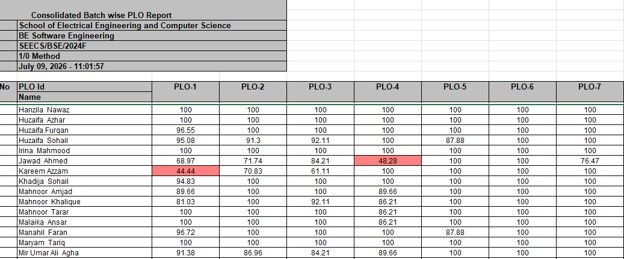
\includegraphics[width=0.8\textwidth]{images/criterion_8/media/PLO1.jpeg}
    \caption{Individual PLO Attainment for Batch2k24}
    \label{fig:sample8}
\end{figure}

The following reports show the Cohort Level Summary of PLO Attainment for Batch 2022 through CLOs, Exit Survey and Internship feedback survey respectively in Figures~\ref{fig:sample9},~\ref{fig:sample10}, and \ref{fig:sample11}.

\begin{figure}[H]
    \centering
    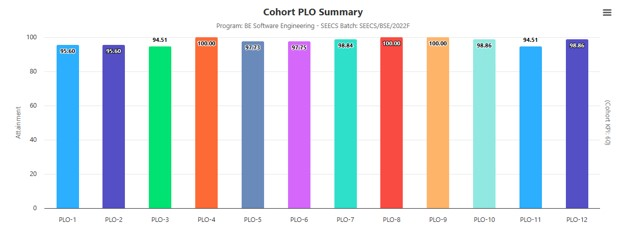
\includegraphics[width=0.8\textwidth]{images/criterion_8/media/Picture2.jpg}
    \caption{Cohort PLO Attainment from CLOs}
    \label{fig:sample9}
\end{figure}

\begin{figure}[H]
    \centering
    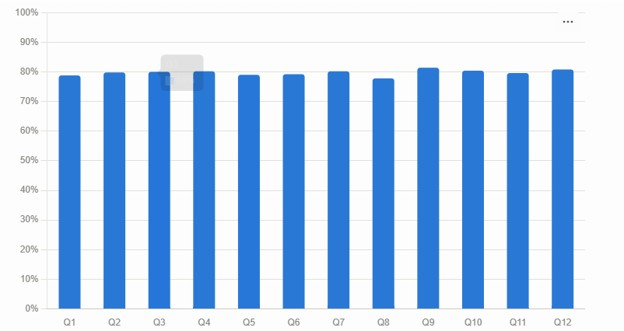
\includegraphics[width=0.8\textwidth]{images/criterion_8/media/Picture4.jpg}
    \caption{Cohort PLO Attainment from Exit Survey}
    \label{fig:sample10}
\end{figure}

\begin{figure}[H]
    \centering
    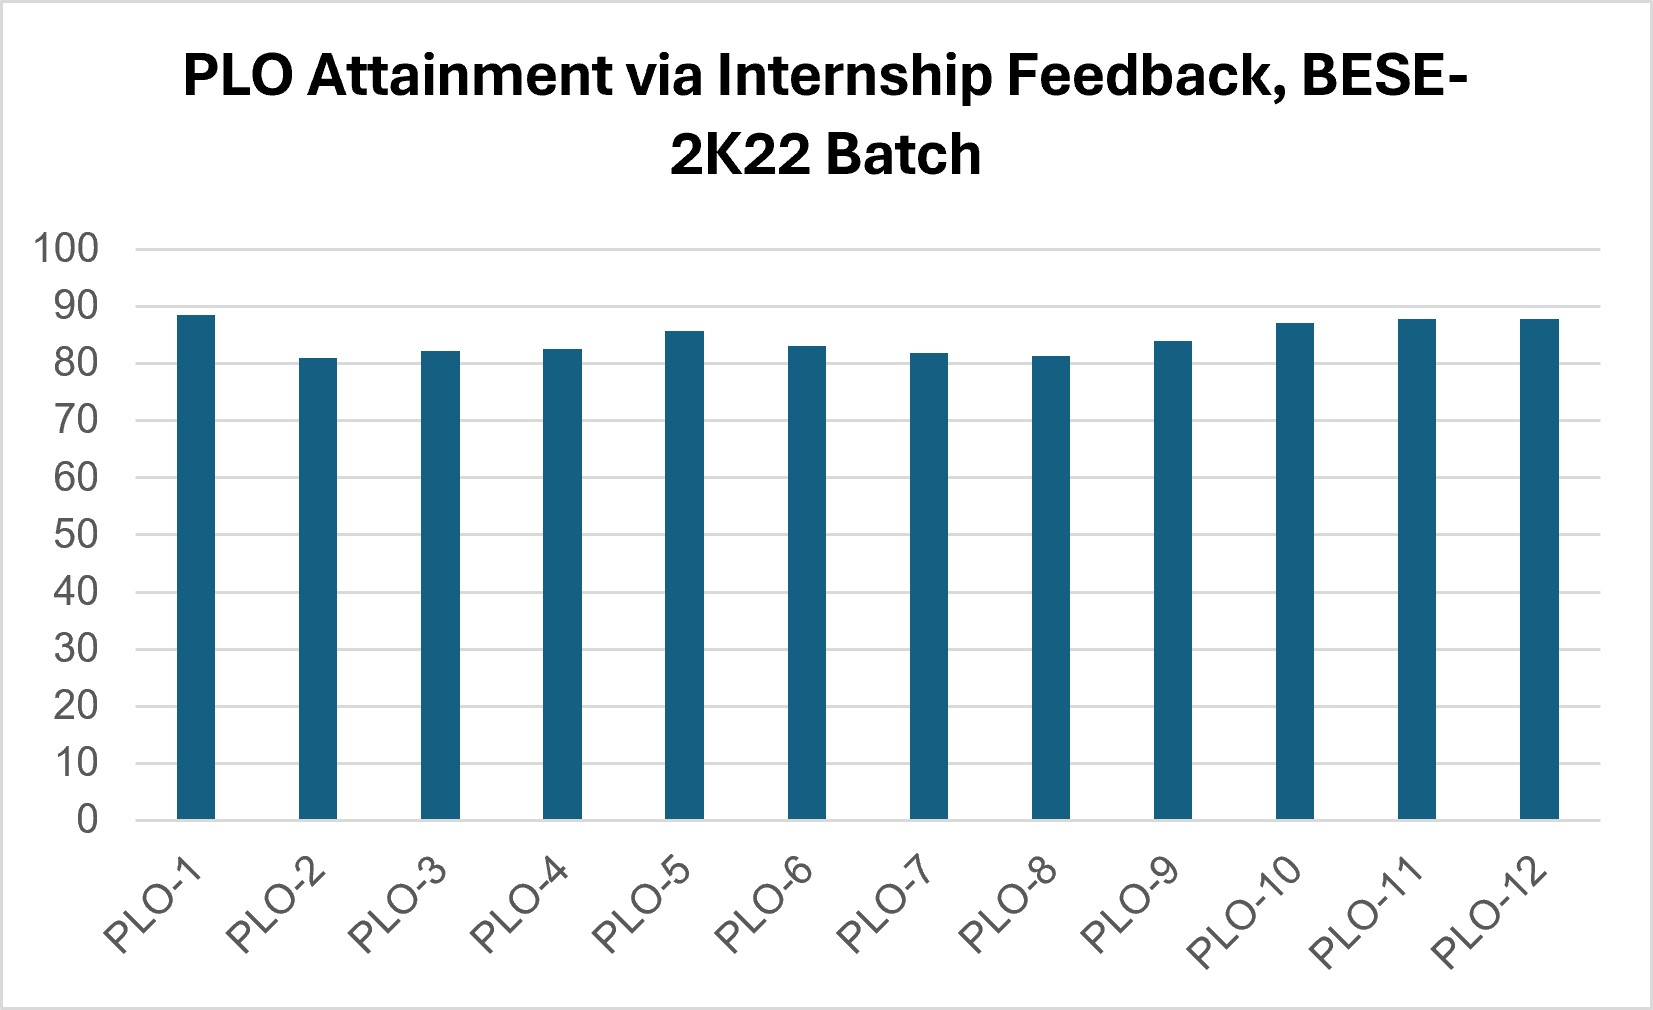
\includegraphics[width=0.8\textwidth]{images/criterion_8/media/Picture5.jpg}
    \caption{Cohort PLO Attainment from Internship Feedback}
    \label{fig:sample11}
\end{figure}

The graphs indicate that the Cohort-Level PLO attainment has achieved the prescribed threshold of 60\% in all three assessments. Accordingly, no CQI intervention is warranted at the cohort level.
Following the observations made by the PEC evaluation team during the previous accreditation visit, the internship feedback forms were reviewed by the Departmental Continuous Quality Improvement (CQI) Committee. The committee analyzed the existing feedback mechanism, considered the evaluators' concerns, and recommended appropriate revisions to improve the effectiveness and comprehensiveness of the internship feedback process. The revised feedback forms were subsequently implemented as part of the department's continuous quality improvement initiatives. The revised system is explained in detail in Criteria 2.

\hypertarget{criterion-8-clos}{%
\section{CLOs}\label{criterion-8-clos}}

\hypertarget{criterion-8-cqi-process-for-clos}{%
\subsection{CQI Process for CLOs}\label{criterion-8-cqi-process-for-clos}}

The innermost loop of OBE implementation model deals with CQI process for CLOs (coursework). The faculty and DLQEC are responsible for CQI of CLOs as shown in Figure~\ref{fig:cqi-clo}. CLOs are directly assessed through coursework and laboratory work involving examination and rubrics. The data is collected, evaluated, and reviewed at the end of every semester. 

\begin{figure}[H]
\centering
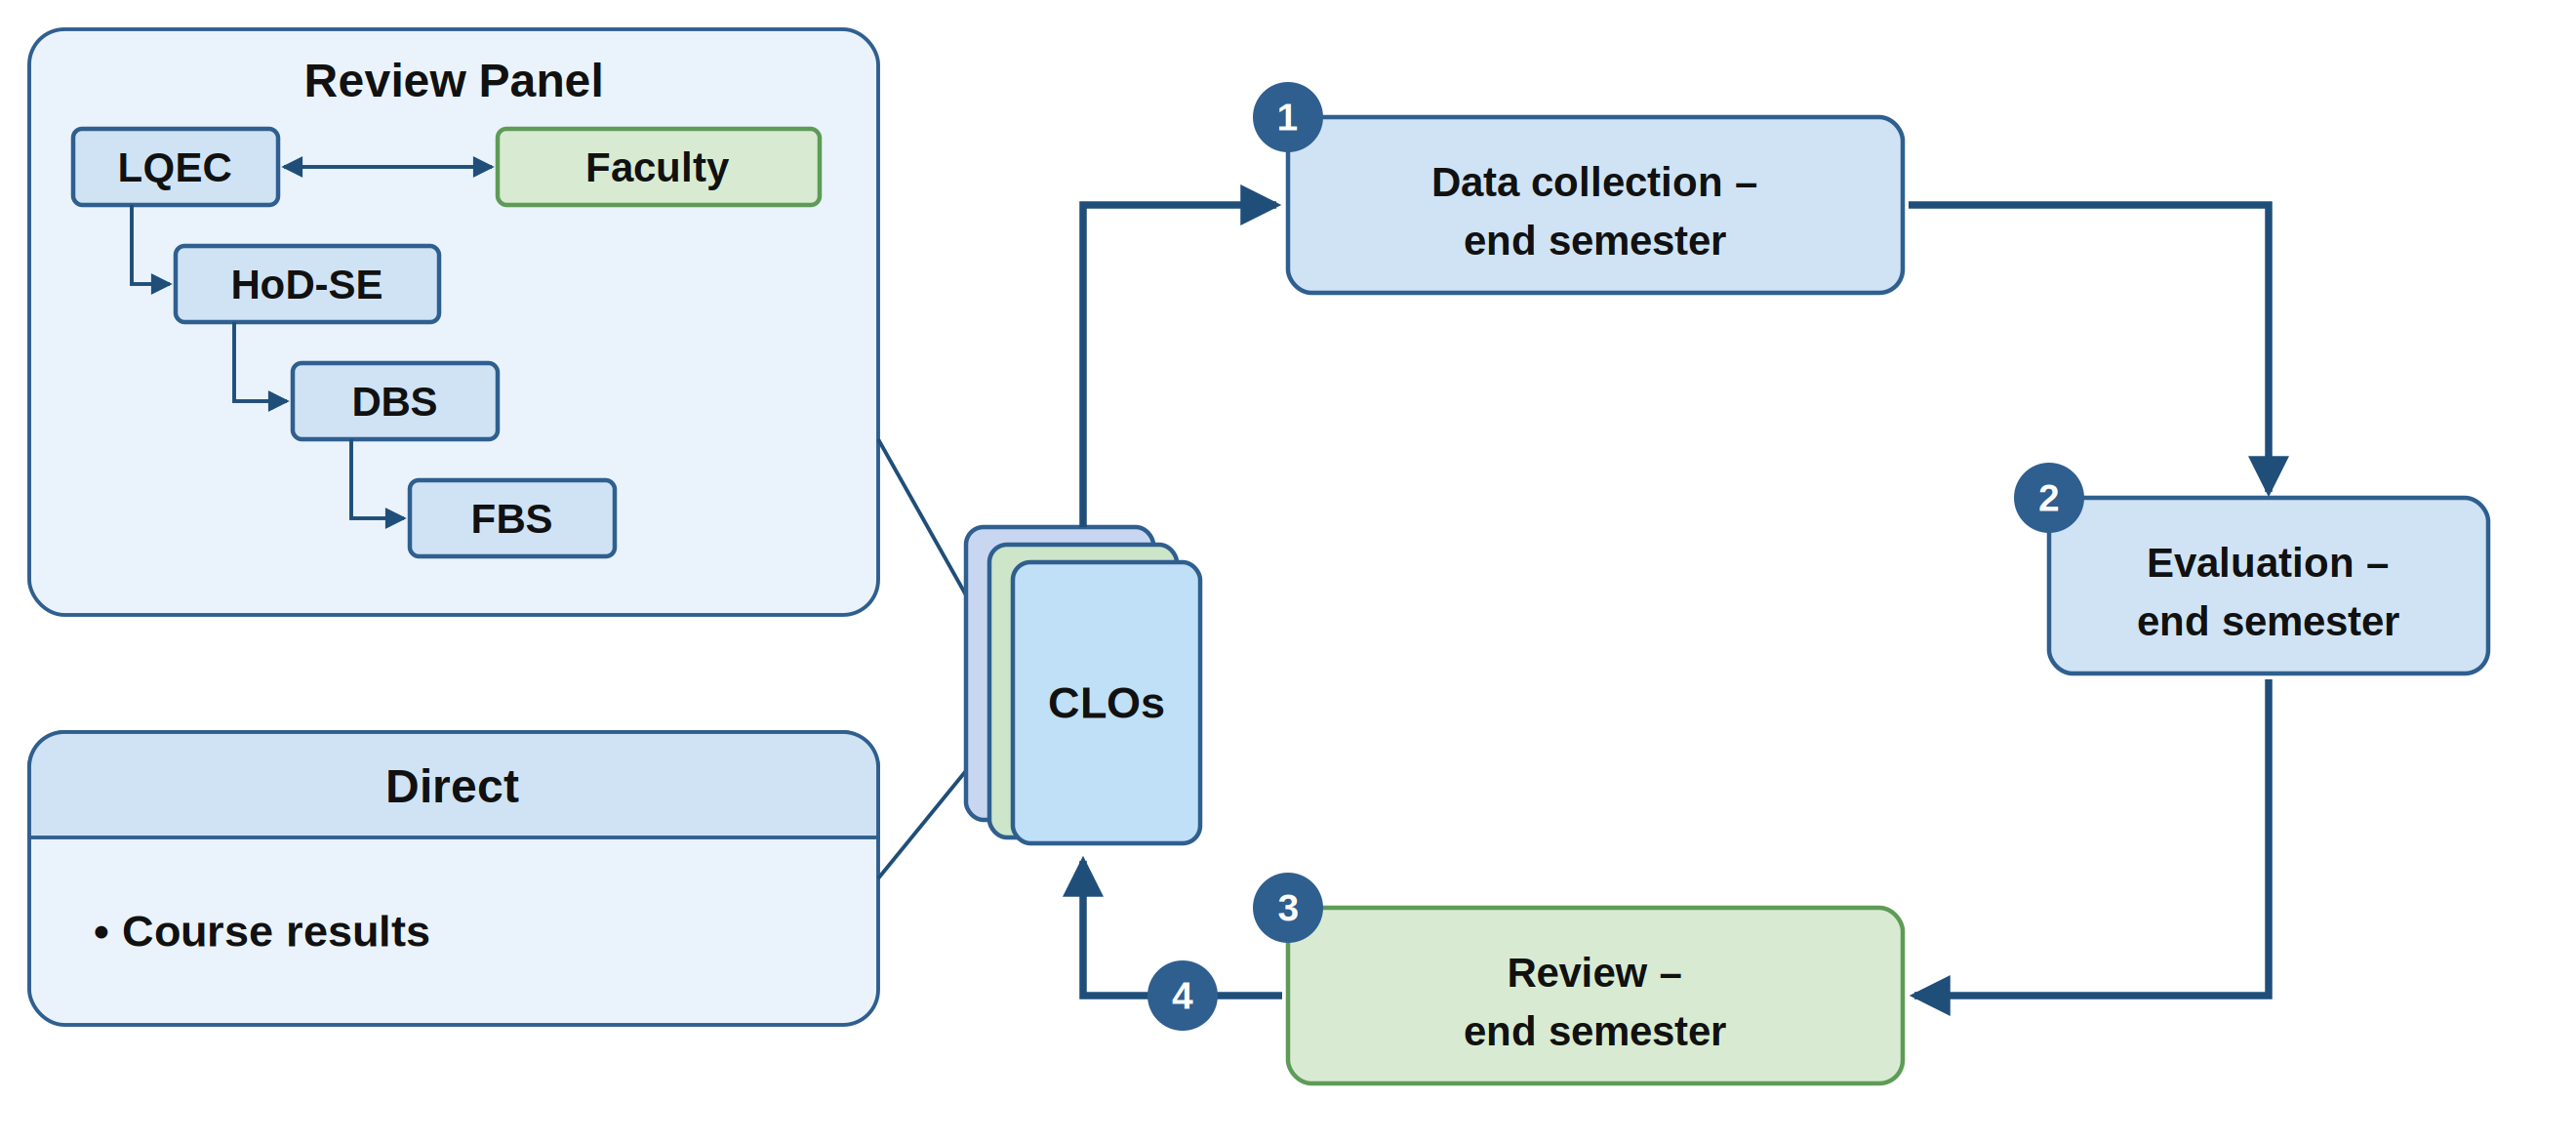
\includegraphics[width=1.0\textwidth]{images/front_matter/media/image-18.png}
\caption{CQI Process for CLOs}
\label{fig:cqi-clo}
\end{figure}

\hypertarget{criterion-8-review-and-corrective-action-processes-for-clos}{%
\subsection{Review and Corrective Action Processes for CLOs}\label{criterion-8-review-and-corrective-action-processes-for-clos}}

Course Learning Outcomes are continuously monitored and evaluated through CLO-attainment analysis and the Course Review Report as part of the department's Continuous Quality Improvement process. The DLQEC reviews Course Learning Outcome attainment, mapping of Course Learning Outcomes to Program Learning Outcomes, Bloom's Taxonomy levels, and learning domains to evaluate the effectiveness of course delivery and assessment. Based on this review, recommendations are made for improvement and are subsequently discussed and approved by the CQI Committee and Departmental Board of Studies. The Knowledge Group Heads also review course outlines, the course materials and taxonomy levels before the start of each semester. Incase of any improvement suggested by the KGH, the improvements are reviewed by CQI committee and corrective actions and initiated through corrective action forms. The approved actions may include revisions to the mapping of Course Learning Outcomes to Program Learning Outcomes, Bloom's Taxonomy levels and assessment methods.
\begin{figure}[H]
\centering
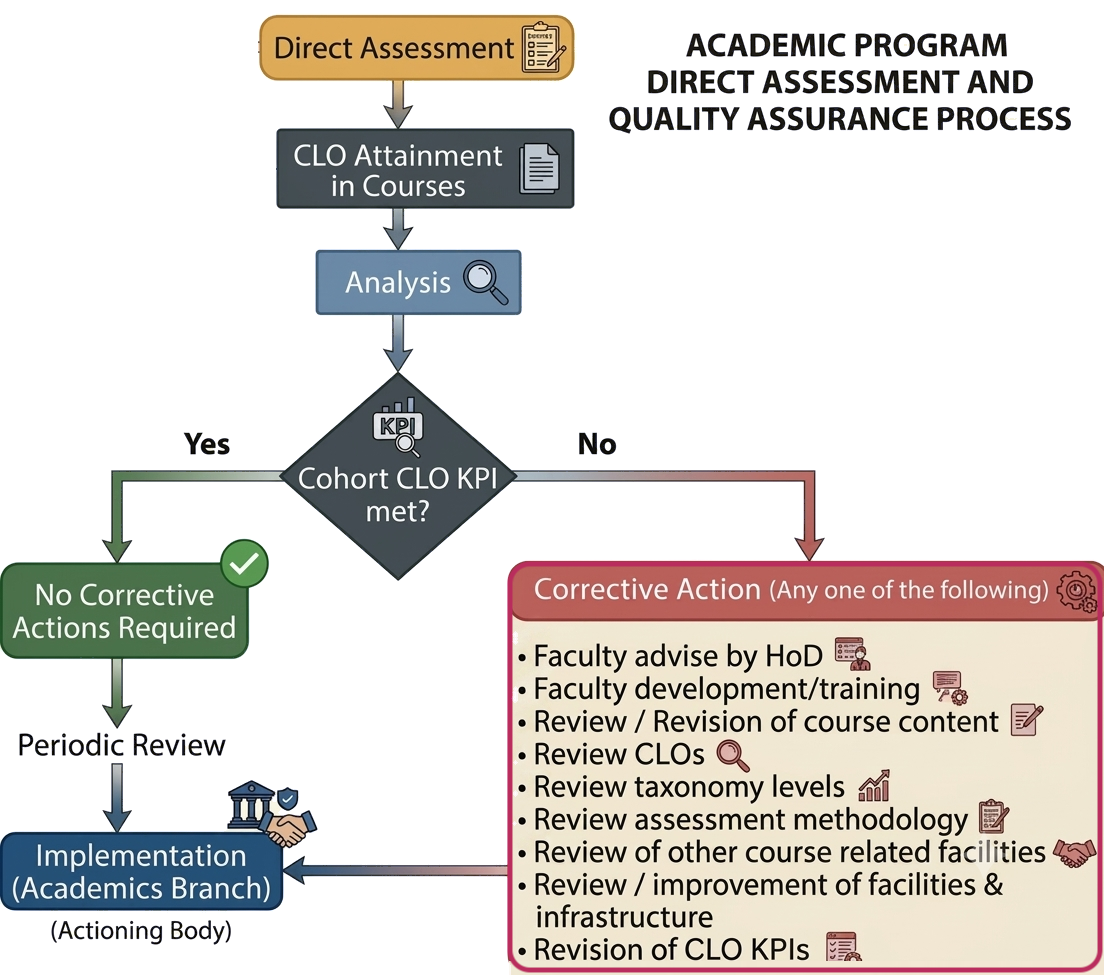
\includegraphics[width=5.18in,height=4.89in]{images/front_matter/media/image-19.png}
\caption{Corrective Actions for CLOs}
\label{fig:corrective-CLOs}
\end{figure}

The Course Learning Outcome review process begins with the measurement of Course Learning Outcome attainment through quizzes, assignments, laboratory work, sessional assessments, and the end-semester examination. Figure~\ref{fig:corrective-CLOs} illustrates the complete process for monitoring and improving Course Learning Outcome attainment. If the cohort-level attainment of a Course Learning Outcome is 60\% or above, the established Key Performance Indicator is considered achieved, and no corrective action is required. However, if the cohort-level attainment falls below 60\%, the Local Quality Enhancement Cell, in consultation with the course instructor and the relevant faculty members, initiates the Continuous Quality Improvement process to identify the underlying causes and recommend appropriate corrective measures. 

Depending on the identified issues, corrective actions may include guidance from the Head of Department, faculty development and training, revision of Course Learning Outcomes, review of Bloom's Taxonomy levels, improvement of assessment methods, enhancement of course delivery practices, and review of laboratory resources and equipment. Nevertheless, if the DLQEC identifies any gaps in CLO coverage, or faculty understanding, appropriate corrective actions are initiated to address the identified shortcomings and further strengthen the effectiveness of the process as part of the department's continuous quality improvement initiatives. The implementation of all the approved corrective actions for improvement of courses is carried out through approval of DBS. Table~\ref{tab:cqi_actions} lists some of the corrective actions taken to improve the CLOs and their mappings.

\begin{table}[ht]
\centering
\footnotesize
\setlength{\tabcolsep}{4pt}
\label{fig:sample12}
\begin{tabular}{
>{\raggedright\arraybackslash}p{4cm}
>{\raggedright\arraybackslash}p{2cm}
>{\raggedright\arraybackslash}p{3cm}
>{\raggedright\arraybackslash}p{2.8cm}
>{\raggedright\arraybackslash}p{3cm}
}
\toprule
\textbf{Observation} &
\textbf{Source} &
\textbf{Action Taken} &
\textbf{Evidence} \\
\midrule
Revision of CLOs &
KGH  &
Updated Course Outline &
Corrective Action form and DBS minutes in Annex ~\ref{annex:oop} \\

Revision of BT Levels &
Faculty Course Review Report &
Revised BT Levels in outline &
Corrective Action form and DBS minutes \\

CLO Coverage &
DLQEC &
Faculty Training and Course Outline Revision &
Meeting Minutes and Training Feedback \\

\bottomrule
\end{tabular}
\caption{Examples of CQI Activities for CLOs}
\label{tab:cqi_actions}
\end{table}

\hypertarget{Stakeholders Feedback Mechanism}{%
\section{Stakeholders Feedback Mechanism}\label{Stakeholders-Feedback-Mechanism}}

Stakeholder engagement is a fundamental component of the Department's Continuous Quality Improvement (CQI) framework. To ensure that the program remains relevant, effective, and aligned with accreditation requirements and industry needs, the Department systematically collects and analyses feedback from students, alumni, employers, faculty members, and the Industrial Advisory Board. Since each stakeholder offers a distinct perspective on program quality, their feedback is incorporated at appropriate decision-making levels to support evidence-based improvements in curriculum, teaching and learning, assessment practices, and overall program management. This structured approach ensures that improvement initiatives are responsive to stakeholder expectations and are continuously monitored for their effectiveness.

\begin{table}[!t]
\centering
\scriptsize                 % Changed from \footnotesize
\renewcommand{\arraystretch}{1.0}   % Reduce row height
\setlength{\tabcolsep}{3pt}         % Reduce column padding
\caption{Stakeholder Inputs and Their Role in Continuous Quality Improvement}

\begin{tabular}{
>{\raggedright\arraybackslash}p{2.6cm}
>{\raggedright\arraybackslash}p{2.6cm}
>{\raggedright\arraybackslash}p{2.5cm}
>{\raggedright\arraybackslash}p{3.8cm}
>{\raggedright\arraybackslash}p{2.6cm}
}
\toprule
\textbf{Stakeholder} &
\textbf{Primary Input} &
\textbf{Decision Level} &
\textbf{CQI Outcome} &
\textbf{Evidence} \\
\midrule

Students &
Course evaluations, student advisory system, exit surveys &
Course and Department Level &
Improvements in course delivery, assessment methods, labs, learning resources and student support &
Survey reports \\
\addlinespace

Faculty &
Course reviews, faculty audit, departmental meetings &
Course and Curriculum Level &
Revision of CLOs, assessment strategies, teaching methods, lab Manuals and course sequencing &
Corrective Action Forms, course review records \\
\addlinespace

Alumni &
Alumni surveys&
Program Level &
Identification of curriculum gaps, emerging skill requirements and enhancement of graduate attributes &
Alumni survey reports\\
\addlinespace

Employers &
Employer surveys, internship evaluations &
Program and Curriculum Level &
Strengthening technical competencies, professional skills, industry alignment and internship improvements &
Employer survey reports, internship feedback reports \\
\addlinespace

Industrial Advisory Board (IAB) &
Recommendations during advisory meetings &
Strategic Program Level &
Curriculum revision, emerging technologies, industry collaboration, new electives and strategic improvements &
Meeting minutes, attendance records, recommendation logs \\
\addlinespace

Pakistan Engineering Council (PEC) &
Accreditation observations and recommendations &
Institutional and Program Level &
Compliance with accreditation requirements, OBE implementation, curriculum restructuring and assessment enhancement &
Accreditation reports, compliance records \\
\addlinespace

Higher Education Commission (HEC) &
Academic policies, curriculum guidelines and quality assurance requirements &
Institutional and Curriculum Level &
Compliance with national policies, credit hour adjustments and curriculum standardization &
HEC policies, implementation records \\
\bottomrule
\end{tabular}

\label{tab:stakeholder_cqi}
\end{table}

\hypertarget{Implementation Plan of Previous Accreditation Observations}{%
\section{Implementation Status of Previous Accreditation Observations}\label{Implementation-Status-of-Previous-Accreditation-Observations}}

The Department is committed to fostering a culture of Continuous Quality Improvement by systematically addressing observations and recommendations from the previous PEC accreditation visit. Since the last evaluation, sustained efforts have been made to strengthen academic and administrative processes, enhance assessment and quality assurance systems, empower faculty through professional development and active participation, and improve overall program effectiveness. The implementation of these corrective actions has been regularly monitored through the department's CQI mechanism. A summary of the implementation status of the observations and the corresponding remedial actions is presented in the Annexure~\ref{annex:rejoinder}.
 \hypertarget{New Facilities Added}{%
\section{New Facilities Added}\label{new-facilities}}

With the completion of the New Academic Block shown in Figure~\ref{fig:sample13}, the Department's infrastructure has been significantly enhanced, providing improved facilities to better support teaching, learning, research, and academic activities for both students and faculty.
\begin{figure}[H]
    \centering
    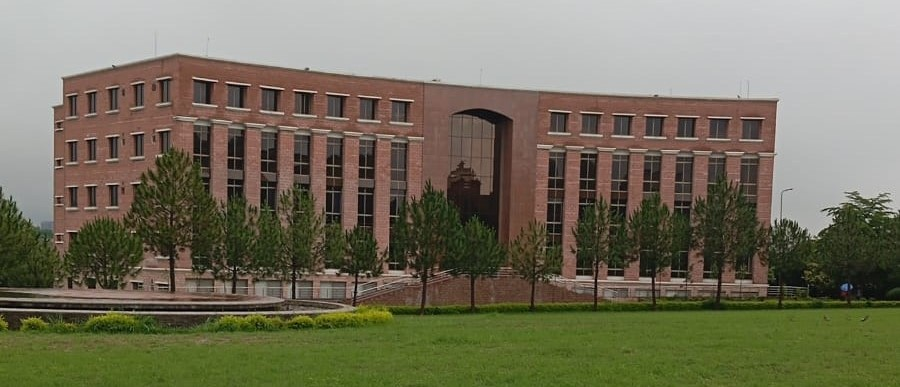
\includegraphics[width=0.6\textwidth]{images/criterion_8/media/acad_block.jpeg}
    \caption{New Academic Block}
    \label{fig:sample13}
\end{figure}

Table~\ref{tab:infrastructure} provides the summary of new facilities added.

\begin{table}[h]
  \centering
  \caption{SEECS infrastructure (existing blocks and New Academic Block)}
  \label{tab:infrastructure}
  \small
  \begin{tabular}{|>{\raggedright\arraybackslash}p{0.39\textwidth}|>{\centering\arraybackslash}p{0.13\textwidth}|>{\centering\arraybackslash}p{0.15\textwidth}|>{\centering\arraybackslash}p{0.10\textwidth}|}
    \hline
    \textbf{Infrastructure} & \textbf{Existing blocks*} & \textbf{New Academic Block} & \textbf{Total} \\
    \hline
    Classrooms                            & 22      & 14      & 36       \\ \hline
    Offices -- Faculty / Officers         & 109     & 26      & 135      \\ \hline
    Principal / Assoc.\ Dean / HoD Offices & 6      & 10      & 16       \\ \hline
    Conference Rooms                      & 3       & 1       & 4        \\ \hline
    Faculty Lounges                       & 2       & 1       & 3        \\ \hline
    Common Rooms (male / female)          & 3       & 2       & 5        \\ \hline
    Exam Branch / Archive Room            & 1       & 1       & 2        \\ \hline
    Other Offices (IT/ACB/Admin/PA)       & 2/2/3/6 & 1/1/1/7 & 3/3/4/13 \\ \hline
  \end{tabular}

  \vspace{2pt}
  {\footnotesize *Existing blocks: UG/PG SEECS blocks, RIMMS and IESE.\par}
  
\end{table}


 \hypertarget{New Initiatives Since Last Accreditation Visit}{%
\section{New Initiatives Since Last Accreditation Visit}\label{new-initiatives}}
The Department has undertaken several strategic initiatives to strengthen the implementation of Outcome-Based Education (OBE) and continuously improve its assessment, evaluation, academic processes, and learning environment. The details of initiatives taken after the last visit are mentioned in the following sections.

\hypertarget{Revised-Assessment-Instruments}{%
\subsection{Revised Assessment Instruments}\label{revised-assesment-instrument}}

\subsubsection{New Alumni Survey (2026)}
The legacy Alumni Survey (9 items, comprising a mix of Likert-scale
and binary Yes/No questions) was fully redesigned following two triggers:
(a) the 2023 PEC accreditation visit flagged poor correlation in PEO-2
and PEO-3 sub-KPI items; and (b) the IAB session held in November 2023
flagged that legacy item 5 inadequately measured PEO-2 attainment.

\begin{itemize}[noitemsep, topsep=0pt]
    \item \textbf{Old form:} 9 items; 4 binary Yes/No questions;
    weak PEO alignment; rigid all-or-nothing pass rule.

    \item \textbf{New form:} 12 items on a 5-point Likert scale (0--4);
    4 items per PEO; each item directly and exclusively mapped to one PEO.

    \item \textbf{Approval trail:} DBS, 20 April 2026
    $\rightarrow$ FBS, 21 April 2026
    $\rightarrow$ IAB endorsement, 5 May 2026.

    \item \textbf{2026 results:} 79 alumni responses;
    PEO-1: 0.803, PEO-2: 0.797, PEO-3: 0.803.
    All three PEOs were attained.
\end{itemize}

\subsubsection{New Employer Survey (2026)}
The Employer Survey was redesigned in parallel with the Alumni Survey.
The revised survey comprises 12 items on a 5-point Likert scale, with
4 items per PEO and an observer-assessment framing. The previous
version contained 7 loosely mapped items. A total of 50 employer
responses were received during the 2026 cycle.

\subsubsection{Redesigned Graduate Exit Survey}
\begin{itemize}[noitemsep, topsep=0pt]
    \item \textbf{Old form:} Generic Likert-scale questions with
    limited traceability to Program Learning Outcomes (PLOs).

    \item \textbf{New form:} Each question is mapped directly to a
    specific PLO. The survey is structured to reduce acquiescence
    bias and is administered through the Learning Management System (LMS).

    \item \textbf{Results:} Batches 2K20, 2K21, and 2K22 consistently
    show mean scores near or above 4.0/5.0 across all PLOs.
\end{itemize}

\subsubsection{Revised Internship Employer Feedback Form}
\begin{itemize} [noitemsep, topsep=0pt]
    \item \textbf{Redesigned:} All items are now mapped to relevant PLOs, providing traceable indirect evidence. 

    \item \textbf{Automated via TMS:} The Online Internship Feedback
    Module, integrated into the Thesis Management System (TMS),
    replaces the previous manual email process.

    \item \textbf{Dual evaluation:} Internships are now assessed through
    both employer feedback submitted via TMS and faculty assessment,
    providing a more comprehensive picture of student performance.
\end{itemize}




\subsection{PLOs Reduced from 12 to 11 (Batch 2K24 Onwards)}
\label{plo-reduction-12-to-11}

The Program Learning Outcomes (PLOs) have been reduced from 12 to 11,
effective from Batch 2K24 onwards, in alignment with the latest PEC
Manual of Accreditation and HEC Undergraduate Education Policy (UEP-2024).
The key structural change involves merging the former PLO-6
(\textit{Engineer and Society}) and PLO-7
(\textit{Environment and Sustainability}) into the revised PLO-6
(\textit{Engineer and the World}).

Table~\ref{tab:plo-revision} summarizes the changes between the previous
PLO framework applicable to batches up to 2K23 and the revised framework
applicable from Batch 2K24 onwards.

\begin{longtable}{|p{0.27\textwidth}|p{0.30\textwidth}|p{0.35\textwidth}|}
\hline
\textbf{Old PLO (till Batch 2K23)} &
\textbf{New PLO (Batch 2K24 and onwards)} &
\textbf{Change} \\
\hline
\endfirsthead

\hline
\textbf{Old PLO (till Batch 2K23)} &
\textbf{New PLO (Batch 2K24 and onwards)} &
\textbf{Change} \\
\hline
\endhead

PLO-1: Engineering Knowledge &
PLO-1: Engineering Knowledge &
Wording streamlined. \\
\hline

PLO-2: Problem Analysis &
PLO-2: Problem Analysis &
Minor update. \\
\hline

PLO-3: Design/Development &
PLO-3: Design/Development &
Unchanged. \\
\hline

PLO-4: Investigation &
PLO-4: Investigation &
Reframed as ``conduct investigation''. \\
\hline

PLO-5: Tool Usage &
PLO-5: Tool Usage &
Unchanged. \\
\hline

PLO-6: Engineer and Society; PLO-7: Environment and Sustainability &
PLO-6: Engineer and the World &
\textbf{Merged:} combines societal and sustainability perspectives. \\
\hline

PLO-8: Ethics &
PLO-7: Ethics &
Expanded to include diversity, inclusion, and international laws. \\
\hline

PLO-9: Teamwork &
PLO-8: Teamwork &
Expanded to include remote and distributed settings. \\
\hline

PLO-10: Communication &
PLO-9: Communication &
Expanded to address cultural and language differences. \\
\hline

PLO-11: Project Management &
PLO-10: Project Management and Finance &
Expanded to include economic decision-making. \\
\hline

PLO-12: Lifelong Learning &
PLO-11: Lifelong Learning &
Expanded to cover learning, adaptability, and critical thinking. \\
\hline
\caption{Comparison of Previous and Revised PLO Frameworks}
\label{tab:plo-revision}\\
\end{longtable}

The revised framework retains the core engineering competencies while
consolidating societal and sustainability considerations into a single
outcome. The remaining outcomes have been renumbered accordingly, with
several also expanded to reflect broader professional and contemporary
engineering requirements.

\subsection{Curriculum Revisions}
\label{subsec:curriculum-revisions}

\subsubsection{Three Working Papers Since Last PEC Visit}
\label{subsubsec:working-papers}

\begin{longtable}{|p{4.0cm}|p{3.5cm}|p{7.5cm}|}
\hline
\textbf{Working Paper} &
\textbf{Applicable From} &
\textbf{Reason / Key Changes} \\
\hline
\endfirsthead

\hline
\textbf{Working Paper} &
\textbf{Applicable From} &
\textbf{Reason / Key Changes} \\
\hline
\endhead

WP No.~30, 64th ACM
\newline 23 January 2023
&
Batch 2K19--2K23
\newline (Fall 2019 onwards)
&
FYDP credit redistribution: 7th semester
from 3 CH to 2 CH, and 8th semester
from 3 CH to 4 CH. This change was
required by NUST's minimum semester
load policy. \\
\hline

WP No.~20, 69th ACM
\newline 6 August 2024
&
Batch 2K24
\newline (Fall 2024 onwards)
&
PEC--HEC UEP-2023 compliance:
English courses added; Pakistan Studies
replaced with Ideology and Constitution
of Pakistan; Ethics introduced for
non-Muslim students; and semester
credit-hour distribution adjusted. PLOs reduced
from 12 to 11.\\
\hline

WP No.~30, 72nd ACM
\newline 4 September 2025
&
Batch 2K25
\newline (Fall 2025 onwards)
&
PEC--HEC UEP-2024 compliance:
compulsory Pakistan Studies and
Fehm-e-Quran-I and II introduced in the
Non-Engineering domain. Engineering electives
increased from 5 to 6. \\
\hline
\end{longtable}


\subsubsection{New and Modified Courses}
\label{subsubsec:new-modified-courses}

\begin{itemize}[noitemsep, topsep=0pt]

    \item \textbf{New Elective --- Virtual and Augmented Reality (CS-365):}
    Introduced to provide students with exposure to extended reality (XR)
    and emerging technologies.

    \item \textbf{New Elective --- Introduction to Quantum Computing:}
    Introduced in response to the recommendation of the Industrial
    Advisory Board (IAB).

    \item \textbf{Fundamentals of Computer Programming (CS-110):}
    Credit hours increased from 3 to 4 CH to strengthen students'
    programming foundations, following IAB recommendations.

    \item \textbf{Engineering Electives:}
    The number of engineering electives increased from 5 to 6,
    providing students with greater flexibility in course selection.

    \item \textbf{Removed Courses:}
    Workshop Practice and Engineering Drawing were removed from the
    common first-year curriculum to sharpen the discipline-specific
    focus.

    \item \textbf{Certification-Style Courses (In Progress):}
    NUST WP No.~2, 73rd ACM, dated 9 February 2026, was approved
    and endorsed at UCAP on 30 January 2026. The initiative will
    recognize 1--3 CH per departmentally validated certification.
    Implementation is awaiting the final Standard Operating
    Procedure (SOP) from the PEC Engineering Accreditation Board.

\end{itemize}


\subsubsection{CEP and OEL Formalised}
\label{subsubsec:cep-oel}

\begin{itemize}[noitemsep, topsep=0pt]

    \item \textbf{Complex Engineering Problems (CEP) Policy:}
    A formal departmental policy has been documented, requiring
    all courses with laboratory work or projects to incorporate
    Complex Engineering Problems.

    \item \textbf{Open-Ended Laboratory (OEL) Activities:}
    Open-Ended Laboratory activities have been institutionalised
    in accordance with PEC requirements. Students define their
    own methodologies, justify their decisions, and validate
    their solutions rather than merely following predefined
    procedures.

\end{itemize}




\subsection{New Internship Mechanism}
\label{subsec:new-internship-mechanism}

\begin{itemize}[noitemsep, topsep=0pt]

    \item \textbf{Mandatory Graduation Requirement:}
    Internship is now compulsory for all BESE students.
    The degree cannot be awarded without successful completion
    of the internship requirement.

    \item \textbf{Automated Process via TMS:}
    The Online Internship Feedback Module has been introduced
    in the Thesis Management System (TMS), replacing the
    previous manual email-based feedback collection process.

    \item \textbf{Dual Evaluation Mechanism:}
    Internship evaluation incorporates both employer feedback
    submitted through TMS and faculty assessment, providing
    a more comprehensive evaluation of student performance.

    \item \textbf{PLO-Aligned Feedback Form:}
    The revised internship feedback form maps each question
    to a specific Program Learning Outcome (PLO), providing
    traceable indirect evidence for assessing PLO attainment.

    \item \textbf{ILO/NPO Coordination:}
    The Industrial Liaison Office (ILO) and NUST Placement
    Office (NPO) maintain a database of industry partners.
    Internship placements are arranged for 100\% of
    undergraduate students, with placements made as close
    to students' homes as possible.

\end{itemize}

\subsection{New PEO Evaluation Framework}
\label{subsec:new-peo-evaluation-framework}

The Program Educational Objectives (PEO) evaluation framework
was comprehensively revised in 2026, replacing the legacy
Key Performance Indicator (KPI) system with a transparent,
multi-step evaluation mechanism based on normalised scoring.

\begin{longtable}{|p{6.2cm}|p{8.8cm}|}
\hline
\textbf{Legacy Framework (Before 2026)} &
\textbf{New Framework (2026)} \\
\hline
9 alumni survey items and 7 employer survey items.
&
12 alumni survey items and 12 employer survey items,
with 4 items mapped to each PEO in each survey. \\
\hline

A combination of Likert-scale and binary Yes/No questions.
&
A uniform 5-point Likert scale, ranging from
0 (Strongly Disagree) to 4 (Strongly Agree). \\
\hline

Rigid evaluation mechanism requiring all sub-KPIs to meet
their respective thresholds individually.
&
A three-step evaluation mechanism:
\begin{enumerate}
    \item Question-level KPI score $\geq 2.0$.
    \item At least 3 out of 4 indicators for each PEO must pass.
    \item Normalised PEO score $\geq 0.60$.
\end{enumerate}
\\
\hline

The binary Yes/No question on pursuing higher education
penalised working graduates who had not pursued further studies.
&
All 8 indicators carry equal weight of 0.25, with no
binary Yes/No items.
\\
\hline

PEO-1 failed to meet the threshold because 36\% of alumni
were pursuing higher education, below the required 50\%
threshold.
&
The 2026 pilot evaluation demonstrated the attainment
of all three PEOs, with normalised scores of 0.803,
0.797, and 0.803, respectively.
\\
\hline
\end{longtable}


\subsection{Infrastructure \& Facilities}
\label{subsec:infrastructure-facilities}

\subsubsection{New Academic Block}
\label{subsubsec:new-academic-block}

A new Academic Block has been completed at SEECS,
significantly expanding the department's physical
infrastructure and providing additional facilities
for teaching, research, administration, and student support.

\subsubsection{Lab Procurement and Upgrades}
\label{subsubsec:lab-procurement-upgrades}

The department has continued to modernise its laboratory
infrastructure through hardware procurement and equipment
upgrades to support teaching, practical learning, and research.

\begin{itemize}[noitemsep, topsep=0pt]

    \item \textbf{Recent Procurement:}
    A total of 45 new personal computers (PCs) were purchased,
    and 50 existing PCs were upgraded with the latest hardware.

    \item \textbf{Lab Equipment Investment:}
    An investment of Rs.~71.55 million was made in 2024--25,
    followed by Rs.~74.82 million in 2025--26, reflecting
    continued investment in laboratory modernisation.

    \item \textbf{Current Laboratory Facilities:}
    The department currently operates 12 computer laboratories,
    one FYDP laboratory, and one Basic Electronics Laboratory.

\end{itemize}


\subsubsection{Network and Connectivity}
\label{subsubsec:network-connectivity}

The department provides network connectivity and computing
facilities to support academic activities, research, and
access to digital resources.

\begin{itemize}[noitemsep, topsep=0pt]

    \item \textbf{Bandwidth:}
    A bandwidth allocation of 910 Mbps is provided through
    PERN via the NUST Campus Core Network, with an additional
    7 Mbps backup connection for research laboratories.

    \item \textbf{Remote Access:}
    A Virtual Private Network (VPN) server hosted at SEECS
    enables secure remote access to campus computing resources.

    \item \textbf{Library Facilities:}
    The library provides high-speed DSL connectivity and Wi-Fi,
    bookable group study rooms, a seminar hall, a conference
    room, and laptop charging points.

\end{itemize}


\subsubsection{Student Support Services: New Initiatives}
\label{subsubsec:student-support-services}

Several initiatives have been introduced to improve student
facilitation, psychological well-being, career development,
and access to support services across NUST.

\begin{itemize}[noitemsep, topsep=0pt]

    \item \textbf{NUST Student Support Services Centre (S3C):}
    A centralised, one-window facilitation platform has been
    introduced to manage student requests and provide access
    to support services across the campus.

    \item \textbf{Centre for Counselling and Career Advisory (C3A):}
    The centre provides professional psychological counselling
    services to the NUST community. Its services include IQ,
    EQ, personality, aptitude, career-interest, stress, and
    depression assessments. The centre is staffed by
    qualified psychologists.

    \item \textbf{Career Development Centre (CDC):}
    The centre provides employability programmes, networking
    events, employer engagement activities, and curriculum
    support. It also coordinates closely with the NUST
    Placement Office to strengthen students' career readiness
    and employment prospects.

\end{itemize}


\subsection{Faculty Development \& Training}
\label{subsec:faculty-development-training}

The department promotes continuous faculty development through
structured training, mentoring, professional development
opportunities, and initiatives aimed at strengthening
Outcome-Based Education (OBE) practices and the academic
environment.

\begin{itemize}[noitemsep, topsep=0pt]

    \item \textbf{OBE Induction:}
    All newly inducted faculty members undergo mandatory pedagogical training (including OBE) at NUST Center for Teaching and Learning (NCTL). The training covers Course Learning Outcome
    (CLO) formulation, Bloom's Taxonomy, and mapping of CLOs
    to Program Learning Outcomes (PLOs).

    \item \textbf{Mentoring System:}
    Each newly inducted faculty member is paired with a
    senior faculty mentor during the first semester to
    facilitate professional integration, teaching support,
    and academic development.

    \item \textbf{Comprehensive OBE Training Sessions:}
    Additional OBE training sessions were conducted following
    the PEC 2023 visit, with particular emphasis on improving
    faculty understanding and application of taxonomy levels
    in teaching, assessment, and outcome evaluation.

    \item \textbf{Green Week:}
    A newly introduced initiative to promote faculty
    well-being and foster a positive, supportive, and
    healthy academic environment.

    \item \textbf{Financial Support for Faculty Development:}
    A dedicated allocation in the university's recurring
    budget supports faculty participation in conferences,
    professional certifications, and pedagogical training.

    \item \textbf{Professional Development Centre (PDC):}
    Established in 2007, the PDC serves as an International
    Finance Corporation (IFC), World Bank Group, management
    training partner and a PEC Continuing Professional
    Development (CPD) partner. It has trained more than
    3,500 professionals from over 450 organisations.

\end{itemize}

\subsection{CQI \& OBE System Enhancements}
\label{subsec:cqi-obe-system-enhancements}

The department has strengthened its Continuous Quality
Improvement (CQI) and Outcome-Based Education (OBE) systems
through formalised quality assurance procedures, enhanced
digital documentation, automated attainment reporting, and
individual student monitoring to ensure continuous
improvement in academic outcomes.

\begin{itemize}[noitemsep, topsep=0pt]

    \item \textbf{Dedicated CQI Committee:}
    A dedicated Continuous Quality Improvement (CQI) Committee
    has been formally established to review assessment results,
    monitor the implementation of corrective actions, and
    facilitate continuous improvement in academic processes
    and programme quality.

    \item \textbf{Enhanced Thesis Management System (TMS):}
    The Thesis Management System (TMS) has been enhanced
    to record and monitor industry-sponsored Final Year
    Design Projects (FYDPs), in addition to managing
    internship feedback. These enhancements provide a
    unified portal for project management and related
    academic monitoring activities.

    \item \textbf{Course and Laboratory Folders on LMS:}
    Mandatory digital documentation of all course and
    laboratory folders on the Learning Management System
    (LMS) ensures the long-term sustainability,
    accessibility, and availability of academic records
    for quality assurance and accreditation purposes.

    \item \textbf{Qalam OBE System:}
    Qalam, NUST's in-house campus management system,
    automatically generates semester-wise and batch-wise
    CLO and PLO attainment reports for all courses.
    These reports support systematic assessment,
    outcome monitoring, and evidence-based academic
    improvement.

\end{itemize}

\subsection{Industry Linkages \& Partnerships}
\label{subsec:industry-linkages-partnerships}

The department maintains strong linkages with industry,
research organisations, and national and international
partners to enhance curriculum relevance, promote
industry-oriented research, and strengthen collaboration
between academia and industry.

\begin{itemize}

    \item \textbf{Industrial Advisory Board (IAB):}
    Multiple IAB sessions were conducted between May 2023 and May 2026, resulting in 11 major recommendations, of which
    7 have been closed. Key completed recommendations
    include the introduction of new electives in Virtual
    and Augmented Reality (VR/AR) and Introduction to
    Quantum Computing, the increase in credit hours for
    Fundamentals of Computer Programming (FoCP), and the
    revision of Program Educational Objective (PEO)
    evaluation instruments.

    \item \textbf{Industry-Sponsored Final Year Design
    Projects (FYDPs):}
    Industry-sponsored FYDPs are co-supervised by SEECS
    faculty members and professionals from startups
    associated with the National Science and Technology
    Park (NSTP). The Thesis Management System (TMS) has
    been enhanced to formally record and monitor these
    projects, supporting systematic tracking and
    coordination.

    \item \textbf{International Research Collaborations:}
    The department maintains research collaborations
    with 81 international collaborators across
    28 countries, strengthening global research
    engagement, knowledge exchange, and opportunities
    for joint academic activities.

    \item \textbf{NUST Industry-Academia Ecosystem:}
    The department benefits from the active ecosystem
    of NUST centres and offices that facilitate
    industry engagement, entrepreneurship, technology
    transfer, research commercialisation, and
    professional development. These include the
    Centre for Advanced Computing (CAC), National
    Science and Technology Park (NSTP), Technology
    Incubation Centre (TIC), Office of Research,
    Innovation and Commercialisation (ORIC),
    Intellectual Property Office (IPO), Technology
    Transfer Office (TTO), Professional Development
    Centre (PDC), Career Development Centre (CDC),
    Industrial Liaison Office (ILO), and Global
    Technology and Technology Network (GTTN).
    Collectively, these entities support stronger
    linkages between academic research, industry
    requirements, entrepreneurship, and graduate
    employability.

\end{itemize}

\subsection{Quick-Reference Summary (All Initiatives)}
\label{subsec:quick-reference-summary}

\small
\renewcommand{\arraystretch}{1.2}

\begin{longtable}{|p{6.7cm}|p{1.8cm}|p{6.5cm}|}
\hline
\textbf{Initiative} & \textbf{Criterion} & \textbf{Status} \\
\hline
\endfirsthead

\hline
\textbf{Initiative} & \textbf{Criterion} & \textbf{Status} \\
\hline
\endhead

Revised Alumni Survey --- 12 items, 4 per PEO, 5-point Likert
& C1 / C8
& DONE --- DBS, FBS, and IAB approved, April--May 2026 \\
\hline

Revised Employer Survey --- 12 items mirroring alumni survey
& C1 / C8
& DONE --- Same approval cycle \\
\hline

New multi-step PEO evaluation (QL-KPI, coverage, normalised score)
& C1 / C8
& DONE --- Piloted in 2026; all 3 PEOs attained \\
\hline

PLOs reduced from 12 to 11 (PLO-6/7 merged; PLO-7 expanded with D\&I)
& C2 / C8
& DONE --- Effective Batch 2K24 onwards \\
\hline

Graduate Exit Survey redesigned (PLO-mapped, bias-reduced)
& C2 / C8
& DONE --- In use \\
\hline

Internship Employer Feedback Form redesigned (PLO-mapped)
& C2 / C3 / C8
& DONE --- Digitised via TMS \\
\hline

Internship made a mandatory graduation requirement
& C3 / C8
& DONE \\
\hline

Internship feedback automated via TMS Online Module
& C3 / C8
& DONE --- Replaces manual email collection \\
\hline

Dual internship evaluation --- employer and faculty
& C3 / C8
& DONE \\
\hline

Curriculum revision WP 64th ACM (2023) --- FYDP credit-hour redistribution
& C3
& DONE --- Batches 2K19--2K23 \\
\hline

Curriculum revision WP 69th ACM (2024) --- UEP-2023 compliance
& C3
& DONE --- Batch 2K24 \\
\hline

Curriculum revision WP No.~20, 69th ACM --- UEP-2024, PLOs 12 to 11
& C3
& DONE --- Batch 2K25 \\
\hline

New elective: Virtual and Augmented Reality (CS-365)
& C3
& ADDED \\
\hline

New elective: Introduction to Quantum Computing
& C3
& ADDED \\
\hline

Fundamentals of Computer Programming (CS-110) credit hours: 3 CH to 4 CH
& C3
& DONE \\
\hline

Engineering electives increased from 5 to 6
& C3
& DONE --- Batch 2K25 \\
\hline

Workshop Practice and Engineering Drawing removed
& C3
& DONE \\
\hline

Certification courses (1--3 CH per certification)
& C1 / C3
& PARTIAL --- Awaiting PEC EAB SOP \\
\hline

Formal CEP Policy documented and distributed 
& C3
& DONE \\
\hline

Open-Ended Laboratory (OEL) activities institutionalised per PEC 
& C3
& DONE \\
\hline

All course and laboratory folders mandated on LMS
& C3 / C8
& DONE \\
\hline

New Academic Block: 14 classrooms, 6 teaching labs, 26 offices
& C6 / C8
& COMPLETED \\
\hline

45 new PCs procured and 50 existing PCs upgraded
& C6
& DONE \\
\hline

Internet: 910 Mbps PERN, 7 Mbps backup, and VPN
& C6
& IN PLACE \\
\hline

S3C --- one-window student support centre
& C4 / C6
& OPERATIONAL \\
\hline

C3A --- professional psychological counselling centre
& C4 / C6
& OPERATIONAL \\
\hline

Career Development Centre (CDC) --- placement and employability
& C4 / C6 / C9
& OPERATIONAL \\
\hline

PDC one-week OBE induction for all newly inducted faculty
& C5 / C8
& ONGOING \\
\hline

Green Week --- faculty well-being initiative
& C8
& DONE \\
\hline

Dedicated CQI Committee established
& C8
& DONE \\
\hline

TMS enhanced to track industry-sponsored FYDPs
& C8 / C9
& DONE \\
\hline

Industry-sponsored FYDPs with NSTP startups
& C9
& ACTIVE \\
\hline

IAB: Multiple sessions (2023--2026), 1 recommendations, 4 closed
& C1 / C9
& ONGOING \\
\hline

International research collaborations: 81 partners across 28 countries
& C9
& ACTIVE \\
\hline

\end{longtable}

\normalsize
\renewcommand{\arraystretch}{1.0}